\documentclass{article}

%%%%%%%%%%%%%%%%%
%%%%%%%%%% PACKAGES
%%%%%%%%%%%%%%%%%
\usepackage{amsfonts}
\usepackage{amsmath}
\usepackage{amsthm}
\usepackage{amssymb}

\usepackage{blindtext}
\usepackage{enumerate}
\usepackage{fancyhdr}
\usepackage{hyperref}
\usepackage[margin=1.5in]{geometry}
\usepackage{multicol}
\usepackage{parskip}
\usepackage{titlesec}

\usepackage[dvipsnames]{xcolor}
\usepackage{graphicx}
\usepackage{pagecolor}
\usepackage{tcolorbox}

\usepackage{pgf}
\usepackage{tikz}
\usepackage{tkz-berge}
\usepackage{pst-node}
\usepackage{tikz-cd} 
\usetikzlibrary{arrows, automata, backgrounds, petri, topaths, shapes}

%%%%%%%%%%%%%%%%%
%%%%%%%%% TCOLORBOX
%%%%%%%%%%%%%%%%%
\tcbuselibrary{theorems}
\tcbuselibrary{skins}
\usepackage{cleveref}

\tcbset{
defstyle/.style={fonttitle=\bfseries\upshape, fontupper=\slshape,
arc=0mm, colback=blue!5!white,colframe=blue!75!black},
theostyle/.style={fonttitle=\bfseries\upshape, fontupper=\slshape,
colback=red!10!white,colframe=red!75!black},
}

\newtcbtheorem[number within=subsection,crefname={definition}{definitions}]{Definition}{Definition}{defstyle}{def}
\newtcbtheorem[use counter from=Definition,crefname={theorem2}{theorems}]{Theorem}{Theorem}{theostyle}{theo}
\newtcbtheorem[use counter from=Definition,crefname={corollary}{corollaries}]{Corollary}{Corollary}{theostyle}{cor}
\newtcbtheorem[use counter from=Definition,crefname={lemma}{lemmas}]{Lemma}{Lemma}{theostyle}{lem}

\newtcbtheorem[use counter from=Definition]{theorem}{Theorem}{theorem style=break,colback=blue!10!white,coltitle=blue!50!black,fonttitle=\upshape\bfseries,fontupper=\itshape,drop fuzzy shadow=blue!50!black!50!white,boxrule=0.1pt, sharpish corners, description delimiters={}{}, separator sign colon, terminator sign={}}{theo}
\newtcbtheorem[use counter from=Definition]{corollary}{Corollary}{theorem style=break,colback=blue!10!white,coltitle=blue!50!black,fonttitle=\upshape\bfseries,fontupper=\itshape,drop fuzzy shadow=blue!50!black!50!white,boxrule=0.1pt, sharpish corners, description delimiters={}{}, separator sign colon, terminator sign={}}{theo}
\newtcbtheorem[use counter from=Definition]{definition}{Definition}{theorem style=plain,enhanced,colframe=blue!50!black,colback=yellow!20!white,coltitle=red!50!black,fonttitle=\upshape\bfseries,fontupper=\itshape,boxrule=0.1pt, sharpish corners, description delimiters={}{}, terminator sign={:}}{theo}
\newtcbtheorem[use counter from=Definition]{lemma}{Lemma}{theorem style=break,colback=Lavender!20,coltitle=Fuchsia,fonttitle=\upshape\bfseries,fontupper=\itshape,drop fuzzy shadow=blue!50!black!50!white,boxrule=0.1pt, sharpish corners, description delimiters={}{}, separator sign colon, terminator sign={}}{theo}

\theoremstyle{plain}
% \newtheorem{lemma}{Lemma}

% \tcolorboxenvironment{lemma}{enhanced jigsaw,colframe=Lavender,interior hidden,before skip=10pt,after skip=10pt, sharpish corners}
\tcolorboxenvironment{proof}{blanker,left=5mm,before skip=10pt,after skip=10pt,borderline west={1mm}{0pt}{Maroon}}

%%%%%%%%%%%%%%%%%
%%%%%%%%%% COMMANDS
%%%%%%%%%%%%%%%%%
\newcommand{\Q}{\mathbb{Q}}
\newcommand{\R}{\mathbb{R}}
\newcommand{\C}{\mathbb{C}}
\newcommand{\Z}{\mathbb{Z}}
\newcommand{\N}{\mathbb{N}}
\newcommand{\T}{\mathcal{T}}
\newcommand{\U}{\mathscr{U}}

\newcommand{\cm}[1]{} % in-line comments
\newcommand{\fakeline}{~\\ \vspace{-1cm}}
\newcommand{\HRule}{\rule{\linewidth}{0.5mm}}
\newcommand{\HRuleRed}{\textcolor{Maroon}{\rule{\linewidth}{0.5mm}}}
\newcommand{\image}[1]{\begin{center}\includegraphics[width=\textwidth]{#1}\end{center}} % full-width image

\newcommand{\ol}[1]{\overline{#1}}
\newcommand{\cyc}[1]{\langle #1 \rangle}

\newcommand{\rainbow}{
\begin{tikzpicture}[x=1mm,y=1mm]
  \colorlet{color min hsb}[hsb]{red}
  \colorlet{color max hsb}[hsb]{magenta}
  \foreach \pos in {0,...,140}{
    \colorlet{my color hsb}[rgb]{color max hsb!\pos!color min hsb}
    \fill[fill=my color hsb,draw=white] (\pos,1) rectangle +(1mm,1mm);
  }
\end{tikzpicture}}

%%%%%%%%%%%%%%%%%
%%%%%%%%%% TITLE INFO
%%%%%%%%%%%%%%%%%
\title{Notes for Abstract Algebra}
\author{Nicholas Tomlin}
\date{\today}

%%%%%%%%%%%%%%%%%
%%%%%%%%% HEADER INFO
%%%%%%%%%%%%%%%%%
\pagestyle{fancy}
\lhead{Nicholas Tomlin}
\chead{}
\rhead{MATH 1530: Abstract Algebra}
\lfoot{}
\cfoot{\thepage}
\rfoot{}

%%%%%%%%%%%%%%%%%
%%%%%%%%%%% TESTING
%%%%%%%%%%%%%%%%%
\newcounter{examplecounter}
\renewcommand{\theexamplecounter}{\arabic{examplecounter}}

\newenvironment{example}[1]{%
\vspace{-0.35cm}
\rule{\linewidth}{0.1mm}

\refstepcounter{examplecounter}%
\noindent\textbf{Example~\theexamplecounter}:}
{\\[0.01in]\rule{\linewidth}{0.1mm}}

%%%%%%%%%%%%%%%%%%%%%%%%%%%%%%%%%%
%%%%%%%%%%%%%%%%%%%%%%%%%%%%%%%%%%
%%%%%%%%%% BEGIN DOCUMENT %%%%%%%%%%%%%
%%%%%%%%%%%%%%%%%%%%%%%%%%%%%%%%%%
%%%%%%%%%%%%%%%%%%%%%%%%%%%%%%%%%%
\begin{document}
% \maketitle
\thispagestyle{empty}
\begin{center}
\textsc{\Large MATH 1530: Abstract Algebra}\\[0.4cm]
\textsc{\large Spring 2017}\\[0.2cm]

\HRuleRed\\[0.4cm]
{ \huge \bfseries Notes for Abstract Algebra: Part I}\\[0.1cm]
\HRuleRed\\[0.2cm]

\Large \textsc{Nicholas Tomlin}
\end{center}
\tableofcontents
\newpage

%%%%%%%%%%%%%%%%%
%%%%%% SECTION: GROUPS
%%%%%%%%%%%%%%%%%
\section{Introduction to groups}
\subsection{Preliminary definitions}

\begin{definition}{}{}
A \textbf{set} is ``a collection of elements," e.g., the integers $\Z = \{\ldots,-2,-1,0,1,2,\ldots\}$, the real numbers $\R$, and the rational numbers $\Q$ (fractions). Note that we use $\Z_{\ge 0} = \{0,1,2,\ldots\}$ to refer to the nonnegative integers.
\end{definition}

\begin{definition}{}{}
If $A,B$ are sets, define the \textbf{Cartesian product} as $$A \times B = \{(a,b) \ | \ a \in A, b \in B\}$$ We can abbreviate $A^2 = A \times A$. Similarly, if $A_1,\ldots,A_n$ are sets, then $$A_1 \times \dots \times A_n = \{(a_1,\ldots,a_n) \ | \ a_1 \in A_1, \ldots, a_n \in A_n\}$$ Let $A^n = A \times \dots \times A$ ($n$ times).
\end{definition}

\begin{definition}{}{}
A \textbf{function} $f : A \rightarrow B$, or a \textbf{map}, is an association of an element $f(a) \in B$ to every element $a \in A$. We call $A$ the \textbf{domain} of $f$, and $B$ the \textbf{codomain} of $f$. Furthermore, the \textbf{range} or \textbf{image} of $f$ is $$\{f(a) : a \in A\}$$
\end{definition}
\begin{example}{}
Let $f : \Z \rightarrow \Z$ be given by $x \mapsto 2x$.\footnote{The symbol $\mapsto$ means "maps to."} The codomain and domain are both $\Z$, while the image is $$\{b \in \Z : b = 2a \text{ for some } a\in\Z \}$$ which is the set of even numbers.
\end{example}

\begin{definition}{}{}
A \textbf{binary operation} on a given set $G$ is a function $* : G \times G \rightarrow G$. For example, integer addition $(+ : \Z \times \Z \rightarrow \Z)$ is a binary operation.
\end{definition}

\subsection{What is a group?}

\begin{definition}{}{}
A \textbf{group} is a set $G$ together with a binary operation $* : G \times G \rightarrow G$ such that the following hold:
\begin{enumerate}[(1)]
\item ``Associativity": for $a,b,c \in G$, $(a*b)*c = a*(b*c)$.
\item ``Existence of the identity": there is an element $e \in G$ such that for all $g \in G$, $e*g = g$ and $g*e = g$.
\item ``Existence of inverses": for every $g \in G$, there is an element that we'll call $g^{-1} \in G$ such that $g*g^{-1}=g^{-1}*g=e$, where $e$ is an identity element of $G$.
\end{enumerate}
\end{definition}

\begin{theorem}{}{}
$(\Z,+)$ forms a group.\footnote{We write the ordered pair $(\Z,+)$ to represent the integers along with the binary operation of addition.}
\end{theorem}

\begin{proof}
Indeed, we check that $(\Z,+)$ satisfies the three axioms of being a group:
\begin{enumerate}[(1)]
\item For associativity, we note that $(a+b)+c = a+(b+c)$ for all $a,b,c \in \Z$.
\item For existence of the identity, $0 \in Z$ satisfies $0 + a = a+0 = a$ for all $a \in \Z$.
\item For existence of inverses, consider some $a \in \Z$. Then assert that $-a \in \Z$ satisfies $a+(-a)=(-a)+a=0$.
\end{enumerate}
Thus, we have shown that $(\Z,+)$ is a group.
\end{proof}

\begin{definition}{}{}
Let $(G,*)$ be a group. Then $G$ is a \textbf{commutative} or \textbf{abelian} group if $a*b = b*a$ for all $a,b \in G$.
\end{definition}

For example, $\Z$, $\R$, and $\Q$ with addition are all \textbf{commutative groups}. However, below is an example of a non-commutative group.

\begin{example}{}{}
Not all groups are commutative. Let $G$ be the symmetries of a can (cylinder) $C$ which are physically possible, i.e., the rigid motions preserving the can. These are called the orientation-preserving isometries of $\R^3$. More precisely, we can define the set of symmetries $$\text{Sym}(C) = \{A : \R \rightarrow \R : \text{ det}(A)=1, A(C)=C \}$$ where $A$ is an linear transformation which is an isometry. Put this together with the binary operation of composition $\circ$, and this forms a group.

However, these motions are not commutative. That is, flipping the can and then rotating it is distinct from rotating the can and then flipping it.
\end{example}

\begin{theorem}{}{}
Every group has a unique identity element.
\end{theorem}

% Section 1.3
\subsection{The group $\Z/n\Z$}
\begin{definition}{}{}
Let $A$ be a nonempty set. Then a \textbf{relation} on $A$ is a subset $R \subseteq A \times A$, which is written $a \sim b$ if and only if $(a,b) \in R$.
\end{definition}
\begin{definition}{}{}
A relation $R$ is an \textbf{equivalence relation} if it satisfies the following three properties:
\begin{enumerate}[(1)]
\item ``Reflexivity": $a \sim a$ for all $a \in A$.
\item ``Symmetry": if $a\sim b$, then $b\sim a$ for all $a,b \in A$.
\item ``Transitivity": if $a\sim b$ and $b\sim c$, then $a\sim c$ for all $a,b,c \in A$.
\end{enumerate}
\end{definition}
Let $f: A \rightarrow D$ be a function. Given $a,b \in A$, we'll say $a\sim b$ if and only if $f(a)=f(b)$. This is an equivalence relation; moreover, all equivalence relations can be written in this form.

\begin{example}{}{}
Consider the set $A = \{\text{students in Math 1530}\}$. For any two students $a,b \in A$, say $a\sim{b}$ if and only if $a$ has the same birthday as $b$. This is an equivalence relation, so we can relate this to the above form as follows. Let $D = \{\text{Jan 1,}\ldots\text{, Dec 31}\}$ be the set of possible birthdays, and $f : A \rightarrow D$ be a function mapping students to their birthdays.
\end{example}
\begin{definition}{}{}
Let $\sim$ be an equivalence relation on $A$. Then we say $$\overline{a} = \{b \in A : a \sim b\}$$ is an \textbf{equivalence class} of $a$. The equivalence classes of $A$ partition it into non-overlapping groups covering all of $A$.
\end{definition}

Let $n \in \Z$. Say $n \mid a$ (pronounced ``$n$ divides $a$") if $a = kn$ for some $k \in \Z.$ Now define a relation $\equiv_n$ on $\Z$ by $a\equiv_nb$ if $n\mid (a-b)$. We call this relation ``congruent modulo $n$." To prove that $\equiv_n$ is an equivalence relation on $\Z$, we must show the following:
\begin{enumerate}[(1)]
\item $a \equiv_na$ for all $a\in\Z$. \cm{Indeed, $a-a=0$ and $n\mid 0$.}
\item $a\equiv_nb$ implies $b\equiv_na$ for all $a,b\in\Z.$
\item $a\equiv_nb$ and $b\equiv_nc$ implies $a\equiv_nc$ for all $a,b,c\in\Z.$
\end{enumerate}
\begin{proof}
Indeed, we will show that $\equiv_n$ satisfies the three axioms of equivalence relations:
\begin{enumerate}[(1)]
\item For reflexivity, $a-a=0$ and $n\mid 0$.
\item For symmetry, $a\equiv_n b \implies n\mid (a-b) \implies a-b=kn$ for some $k\in\Z$. We want to show that $b\equiv_n a$, i.e., $b-a=ln$ for some $l\in\Z$. We may take $l=(-k)$.
\item For transitivity, there exists $k,l\in\Z$ such that $a-b=kn$ and $b-c=ln$. Then, adding these equations gives $a-c=(k+l)n$. Since $(k+l)\in\Z$, we conclude $n\mid (a-c) \implies a\equiv_nc$.
\end{enumerate}
\end{proof}

\begin{definition}{}{}
$\Z/n\Z$ is the set of equivalence classes modulo $n$, i.e., equivalence classes with respect to the equivalence relation $\equiv_n$.
\end{definition}

For example, $\Z/5\Z = \{\overline{0}, \overline{1}, \overline{2}, \overline{3}, \overline{4}\}$. The choice of ``captains" is not important, so we could alternatively write this as $\Z/5\Z = \{ \ol{10}, -\ol{4}, \ol{2}, \ol{8}, \ol{24} \}$.
\begin{definition}{}{}
We define the binary operation of addition $+: \Z/n\Z \times \Z/n\Z \rightarrow \Z/n\Z$ as follows: $\overline{a}+\overline{b} = \overline{a+b}$ for all $\overline{a}, \overline{b} \in \Z/n\Z$.
\end{definition}
\begin{lemma}{}{}
Addition on $\Z/n\Z$ is well-defined, as stated above.
\end{lemma}
\begin{proof}
Given $a_1,a_2 \in \Z$ such that $\overline{a}_1 = \overline{a}_2$ and $b_1,b_2 \in \Z$ such that $\overline{b}_1 = \overline{b}_2$, we want to show that $\overline{a_1+b_1} = \overline{a_2+b_2}$. Indeed, $a_1-a_2 = kn$ and $b_1-b_2 = ln$ for $k,l\in\Z$. Adding these equations gives $$(a_1+b_1) - (a_2+b_2) = (k+l)n$$ so that $\overline{a_1+b_1} = \overline{a_2+b_2}$ since $(k+l)\in\Z$.
\end{proof}
\begin{theorem}{}{}
$(\Z/n\Z, +)$ is a group.
\end{theorem}
\begin{proof}
Again, we check the three group axioms:
\begin{enumerate}[(1)]
\item We have 
\begin{align*}
\overline{a}+(\overline{b}+\overline{c}) &= \overline{a} + \overline{b+c} \\
&= \overline{a + (b+c)} \\
&= \overline{(a+b) +c} \\
&= \overline{a+b} + \overline{c} \\
&= (\overline{a} + \overline{b}) + \overline{c}
\end{align*}
by associativity of addition.
\item We have $\overline{0} + \overline{a} = \overline{a} + \overline{0} = \overline{a}$ for all $a \in \Z/n\Z$.
\item We have $-\overline{a} + \overline{a} = \overline{a} + (-\overline{a}) = \overline{0}$ for all $a \in \Z/n\Z$.
\end{enumerate}
\end{proof}
\begin{definition}{}{}
We define the binary operation of multiplication $\cdot: \Z/n\Z \times \Z/n\Z \rightarrow \Z/n\Z$ as follows: $\overline{a}\cdot \overline{b} = \overline{ab}$ for all $\overline{a}, \overline{b} \in \Z/n\Z$.
\end{definition}
\begin{theorem}{}{}
Multiplication on $\Z/n\Z$ is well-defined, as defined above.
\end{theorem}

\subsubsection{The multiplicative group $(\Z/n\Z)^{\times}$}
However, $(\Z/n\Z, \cdot)$ is not a group unless $n=1$, as inverses may not exist. Indeed, $\bar{1}$ is an identity, but $\bar{0}\cdot a = \bar{1}$ has no solution, i.e.,  there is no multiplicative inverse for $\bar{0}$. Now, let: $$(\Z/n\Z)^{\times} = \{ \bar{a} \in \Z/n\Z : \bar{a}\cdot\bar{c} = \bar{1} \text{ for some } \bar{c}\in\Z/n\Z \}$$
We call this set ``the multiplicative units of $\Z/n\Z$."

\begin{example}{}{}
Given $n=4$, we say $(\Z/4\Z)^{\times} = \{ \bar{1}, \bar{3} \}$. In particular, $\bar{1} \cdot \bar{1} = \bar{1}$ and $\bar{3} \cdot \bar{3} = \bar{1}$.
\end{example}
\begin{theorem}{}{}
$((\Z/n\Z)^{\times}, \cdot)$ is a group.
\end{theorem}
\begin{proof}
Given $\bar{a}, \bar{c} \in (\Z/n\Z)^{\times}$, we must show that $\bar{a} \cdot \bar{c} \in (\Z/n\Z)^{\times}$. First, we will show that $\cdot$ defines a binary operation on $(\Z/n\Z)^{\times}$, i.e., ($\Z/n\Z)^{\times}$ is closed under multiplication. Indeed, $\bar{a} \cdot \bar{b} = \bar{1}$ and $\bar{c} \cdot \bar{d} = \bar{1}$ for some $\bar{b}, \bar{d} \in \Z/n\Z$. Multiplying these equations gives:
\begin{align*}
\bar{1} &= (\bar{a}\cdot\bar{b})(\bar{c}\cdot\bar{d}) \\
&= (\bar{a}\cdot\bar{c})(\bar{b}\cdot\bar{d})
\end{align*}
In addition, associativity holds as in $\Z/n\Z$. There is an identity element, namely $\bar{1}$, and inverses exist as in $\Z/n\Z$ based on the definition of $(\Z/n\Z)^{\times}$.
\end{proof}
\begin{theorem}{}{}
$(\Z/n\Z)^{\times} = \{ \bar{a} : a \in \Z, (a,n) = 1 \}$
\end{theorem}
\subsubsection{Applications of arithmetic in $\Z/n\Z$}
\begin{example}{}{}
\textit{What is the last digit of $2^{50}$?} To calculate this, work in $\Z/10\Z$:
\begin{align*}
\bar{2} \cdot \bar{2} &= \bar{4} \\
\bar{2} \cdot \bar{2} \cdot \bar{2} &= \bar{8} \\
\bar{2} \cdot \bar{2} \cdot \bar{2} \cdot \bar{2} &= \bar{6} \\
\bar{2} \cdot \bar{2} \cdot \bar{2} \cdot \bar{2} \cdot \bar{2} &= \bar{2}
\end{align*}
and so on. Hence this cycles through ($\bar{2}, \bar{4}, \bar{8}, \bar{6}$) as demonstrated above. We can use this pattern to see the last digit is \boxed{4}. Alternatively, since $\overline{2^5} = \bar{2}$:
\begin{align*}
\overline{2^{50}} &= \overline{(2^5)^{10}} \\
&= \overline{2^{10}} \\
&= \overline{2^5} \cdot \overline{2^5} \\
&= \bar{2} \cdot \bar{2} = \bar{4}
\end{align*}
\vspace{-0.8cm}
\end{example}
% 1.4
\subsection{Some general theorems about groups}
\begin{lemma}{}{}
Let $(G, *)$ be a group. Then $G$ has a unique identity element.
\end{lemma}
\begin{proof}
Let $e,f \in G$ be identity elements. Then:
\begin{align*}
e = e*f &\text{ (since $f$ is an identity element)} \\
e*f = f &\text{ (since $e$ is an identity element)}
\end{align*}
Therefore $e=f$ and there is exactly one identity element.
\end{proof}
\begin{lemma}{}{}
Let $(G, *)$ be a group. Then $G$ has a unique inverse.
\end{lemma}
\begin{proof}
Given $a \in G$, suppose that $b,c \in G$ are inverses of $a$. Then:
\begin{align*}
e &= a*b \text{ (since $b$ inverse of $a$)} \\
c*e &= c*a*b \\
c &= b \text{ (since $c$ inverse of $a$)}
\end{align*}
Since $b=c$, every element of a group must have a unique inverse.
\end{proof}
\begin{lemma}{}{}
Let $(G, *)$ be a group. Then $(a*b)^{-1} = (b^{-1})*(a^{-1})$ for all $a,b \in G$.
\end{lemma}
\begin{proof}
We need to check that $(a*b)*((b^{-1})*(a^{-1})) = e$ is the identity element. This is left as an exercise to the reader.
\end{proof}
\begin{lemma}{}{}
Let $(G, *)$ be a group. For any $a_1,\ldots,a_n \in G$, $a_1*\dots *a_n$ has a well-defined value, i.e., is independent of bracketing.
\end{lemma}
\begin{theorem}{}{}
Given $(G, *)$ a group and $a,b \in G$, the equation $ax=b$ has a unique solution.
\end{theorem}
\subsection{The order of a group}
\begin{definition}{}{}
Let $(G,*)$ be a group. The \textbf{order of a group} $G$ denoted $|G|$ is the number of elements. If $G$ is infinite, say $|G| = \infty$.
\end{definition}
\begin{definition}{}{}
Let $(G,*)$ be a group. The \textbf{order of an element} $a \in G$ is the smallest $n \in \Z_{> 0}$ such that $a^n = e$. 
\end{definition}
\begin{example}{}{}
The symmetries of a can $Sym(C)$ has order $|Sym(C)| = \infty$, but it has elements of finite order. For instance, the identity has order $|e| = 1$. A rotation by $180^{\circ}$ has order $2$, a rotation by $120^{\circ}$ has order $3$, and so on. In fact, for any order $n \in \Q$, a rotation by $2\pi/n$ has order $n$.
\end{example}

\subsection{A brief interlude on functions}
\begin{definition}{}{}
Let $f : A \rightarrow C$ be a function on sets. Then $f$ is \textbf{injective} (one-to-one) if given any two elements $a,b \in A$, then $f(a)=f(b) \implies a=b$.\footnote{The contrapositive, $a \ne b \implies f(a) \ne f(b)$ is equivalent.}
\end{definition}
\begin{definition}{}{}
Let $f : A \rightarrow C$ be a function on sets. Then $f$ is \textbf{surjective} (onto) if for all $c\in C$, there exists $a\in A$ with $f(a)=c$.
\end{definition}
\begin{definition}{}{}
A function is \textbf{bijective} if it is both injective and surjective.
\end{definition}
Given a function $f : A \rightarrow C$ between finite sets $A$ and $C$, then we write $|A|$ to denote the number of elements (i.e., the \textbf{cardinality}) of $A$. Then, we can say:
\begin{enumerate}
\item $f$ injective $\implies |A| \le |C|$
\item $f$ surjective $\implies |A| \ge |C|$
\item $f$ bijective $\implies |A| = |C|$
\end{enumerate}

\subsection{Dihedral groups}
\begin{definition}{}{}
The \textbf{dihedral group}, denoted $D_{2n}$, is the group of rigid motions of a regular $n$-gon. The group operation is composition.
\end{definition}
The $2n$ subscript in the name for the dihedral group refers to the order of the group. We can rotate the $n$-gon by integer multiples of $2\pi/n$, and we can ``flip" the $n$-gon in $\R^3$. These combinations of rotations and flips are specifically the $2n$ elements of the dihedral group.

More rigorously, we can label the vertices of an $n$-gon $\{1,\ldots,n\}$ in clockwise order. A rigid motion of the $n$-gon can be recorded as a bijection $$\sigma : \{1,\ldots,n\}\rightarrow\{1,\ldots,n\}$$
i.e., a permutation of $\{1,\ldots,n\}$. Therefore, $\sigma(j)$ records the new position of vertex $j$. We claim that the map of sets $$D_{2n}\rightarrow \{\text{bijections from } \{1,\ldots,n\} \rightarrow \{1,\ldots,n\}\}$$
is injective. The intuition here is that the rigid motions of the $n$-gon are a subset of the possible permutations. Now, note that $D_{2n}$ has at least $2n$ elements (as shown above).
\begin{theorem}{}{}
$|D_{2n}| = 2n$ (i.e., $D_{2n}$ is the dihedral group of order $2n$)
\end{theorem}
\begin{proof}
We know that $|D_{2n}| \ge 2n$, so we want to show $|D_{2n}| \le 2n$. Define a map:
\begin{align*}
D_{2n} &\rightarrow \{ (1,2),\ldots,(n-1,n), (n,1), (2,1), \ldots, (n,n-1), (1,n) \} \\
\sigma &\mapsto (\sigma(1), \sigma(2))
\end{align*}
where the target has cardinality $2n$. This map is injective, since any two adjacent elements uniquely define a rigid motion of the $n$-gon. Thus, $|D_{2n}| \le 2n$.
\end{proof}

\subsubsection{Explicit description of $D_{2n}$}

Label an $n$-gon $\{1,\ldots,n\}$ on its vertices. Let $r$ be clockwise rotation by $2\pi/n$, and let $s$ be a reflection about the central line bisecting the angle at vertex $1$. Note that:
\begin{itemize}
\item $1, \ldots, r^{n-1} \in D_{2n}$ are distinct rotations.
\item $s$ is distinct from $1, \ldots, r^{n-1}$.
\item $s,sr,sr^2,\ldots,sr^{n-1} \in D_{2n}$ are all distinct.
\end{itemize}
\begin{theorem}{}{}
$D_{2n} = \{1,\ldots,r^{n-1}, s, \ldots, sr^{n-1}\}$
\end{theorem}
\begin{proof}
We need only show that $$r^i \ne sr^j \text{ for any } i,j \in \{1,\ldots,n-1\}$$ Indeed, $r^{i-j} \ne s$.
\end{proof}
Furthermore, $rs = sr^{-1}$, i.e., rotating and reflecting is the same as reflecting and rotating by the same amount in the opposite direction.

Given these observations, we now know how to multiply in $D_{2n}$. For example, we can multiply the rigid motions $(sr^6)$ and $(sr^9)$ on an arbitrary regular $n$-gon:
\begin{align*}
(sr^6)(sr^9) &= s(r^6s)r^9 \\
&= s(r^5sr^{-1})r^9 \\
&= s(sr^{-6})r^9 \\
&= r^3
\end{align*}
Alternatively, we can define $D_{2n}$ in terms of generators and relations as follows:
$$D_{2n} = \langle r,s \ | \ r^n = 1, s^2 = 1, rs=sr^{-1} \rangle$$
In particular, any relation on elements of $D_{2n}$ can be obtained from the given relations.

\subsection{Symmetric groups}
\begin{definition}{}{}
Let $X$ be a non-empty set, and let $S_X$ be the permutations of $X$. When $X = [n] := \{1,\ldots,n\}$, we write $S_n = S_{\{1,\ldots,n\}}$. Then $S_X$ is a group under composition, where $f*g = g\circ f$.
\end{definition}
\begin{example}{}{}
$S_3 = \{\{1,2,3\}, \{1,3,2\}, \{2,1,3\}, \{2,3,1\}, \{3,1,2\}, \{3,2,1\}\}$.
\end{example}
\begin{lemma}{}{}
A map $f : A \rightarrow C$ is a bijection if and only if there exists a function $g : C \rightarrow A$ such that $f\circ g = \operatorname{id}_C$ and $g\circ f = \operatorname{id}_A$.
\end{lemma}

\begin{theorem}{}{}
The order $|S_n| = n!$, i.e., the factorial of $n$.
\end{theorem}
\begin{proof}
To choose a permutation of $\{1,\ldots,n\}$, we can choose any of $n$ mappings for $1$, $n-1$ remaining mappings for $2$, and so on. Since there is no ``overlap,'' this is an injective function. Furthermore, since this is injective and the domain and range have the same number of elements, it is also a bijection.
\end{proof}

\subsubsection{Cycle notation for permutations}
Let $\sigma \in S_n$. Using the two-line notation style for permutations, we can write:
$$\sigma = \begin{pmatrix}
1 & 2 & 3 & 4 & 5 & 6 & 7 \\
7 & 2 & 4 & 1 & 6 & 5 & 3
\end{pmatrix}$$
This maps $1\mapsto 7$, $2\mapsto 2$, and so on. Alternatively, it can be represented with a directed graph, as in the following example:

\begin{example}{}{}
Given $\sigma = \{7 , 2 , 4 , 1 , 6 , 5 , 3\}$, the corresponding directed graph is as follows:
\begin{center}
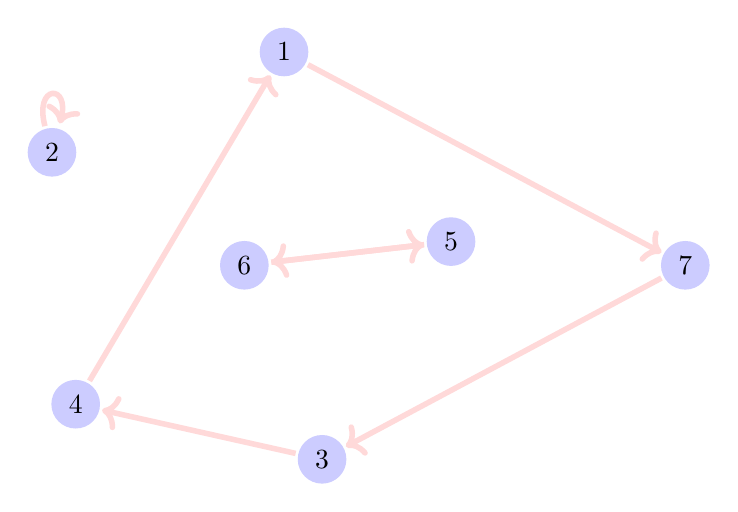
\begin{tikzpicture}[line width=2pt, scale=0.7] 
	\tikzstyle{every node} = [circle, fill=blue!20]
	\node (1) at (0.72, 3.87) {1};
	\node (4) at (-3.06, -2.52) {4};
	\node (3) at (1.41, -3.52) {3};
	\node (2) at (-3.49, 2.05) {2};
	\node (5) at (3.75, 0.43) {5};
	\node (6) at (0,0) {6};
	\node (7) at (8,0) {7};
	\draw [->, pink!60] (1)--(7);
	\draw [->, pink!60] (7)--(3);
	\draw [->, pink!60] (3)--(4);
	\draw [->, pink!60] (4)--(1);
	\draw [->, pink!60] (5)--(6);
	\draw [->, pink!60] (6)--(5);
	\path (2) edge [pink!60, loop above] (2);
\end{tikzpicture}
\end{center}
The above directed graph can be divided into three disjoint cycles $\sigma = (1734)(56)(2)$, or just $\sigma = (1734)(56)$.\footnote{It is a convention to remove $1$-element cycles from the notation, just as a convenience. The order of these cycles is not important, and $\sigma$ could equivalently be written as $\sigma = (65)(3417)$, or one of many other possible combinations.} More generally, we'll claim that any such permutation must produce a graph of disjoint cycles. This notation allows us to calculate inverses and powers:
\begin{itemize}
\item \textbf{Inverses} - $\sigma^{-1} = (4371)(65)$, which is calculated by going in the reverse direction
\item \textbf{Powers} - $\sigma^{2} = (13)(47)(5)(6) = (13)(47)$, where we count every other element of each cycle. To calculate $\sigma^{n}$, count every $n$th element.
\end{itemize}
\fakeline
\end{example}
\begin{theorem}{}{}
Let $\sigma \in S_n$. Then, draw an arrow from $i$ to $\sigma(i)$ for each $i \in \{1,\ldots,n\}$. The resulting directed graph is a collection of disjoint cycles.
\end{theorem}
\begin{theorem}{}{}
In general, for $\sigma \in S_n$, $|\sigma|$ is the least common multiple of all cycle lengths in the cycle decomposition of $\sigma$.
\end{theorem}
\begin{definition}{}{}
Say that $\sigma \in S_n$ is an \textbf{m-cycle} if its cycle notation has just one cycle of length $m$ (and all other cycles length $1$).
\end{definition}
We can also use this notation to calculate products (i.e., composition) of permutations. For example, consider the case of $(154)(23) \circ (12345)$:\footnote{$\sigma \circ \tau$ means first $\tau$, then $\sigma$} since $1 \mapsto 2$ in $(12345)$ and then $2\mapsto 3$ in $(154)(23)$, it must be the case that $1\mapsto 3$ in their composition. This general principle can be applied repeatedly to calculate that
\begin{align*}
(154)(23) \circ (12345) &= (13)(2)(4)(5) = (13) \\
(1734) \circ (56) &= (1734)(56)
\end{align*}
where in the second example, composition is nothing more than concatenation since the two permutations are non-overlapping. Such disjoint cycles always commute, but not all permutations commute. For example, $(12) \circ (13) = (132)$ but $(13) \circ (12) = (123)$.
\begin{theorem}{}{}
$S_n$ is nonabelian for $n \ge 3$.
\end{theorem}
\subsection{Homomorphisms and isomorphisms}
\subsubsection{Motivation}
Consider the following groups:
\begin{enumerate}[1.]
\item $(\Z/2\Z,+) = \{\bar{0}, \bar{1}\}$
\begin{multicols}{2}
\begin{itemize}
\item $\bar{0}+\bar{0}=\bar{0}$
\item $\bar{0}+\bar{1}=\bar{1}$
\end{itemize}
\begin{itemize}
\item $\bar{1}+\bar{0}=\bar{1}$
\item $\bar{1}+\bar{1}=\bar{0}$
\end{itemize}
\end{multicols}
\item $S_2 = \{ \text{id}, (12) \}$, with $\circ$:
\begin{multicols}{2}
\begin{itemize}
\item $\text{id}\circ\text{id}$ = id
\item $\text{id}\circ(12) = (12)$
\end{itemize}
\begin{itemize}
\item $12\circ\text{id}=(12)$
\item $(12)\circ(12)=\text{id}$
\end{itemize}
\end{multicols}
\item A group $(P,+)$ with elements $P = \{\text{even, odd}\}$, with $+$ given by:
\begin{multicols}{2}
\begin{itemize}
\item even + even = even
\item even + odd = odd
\end{itemize}
\begin{itemize}
\item odd + even = odd
\item odd + odd = even
\end{itemize}
\end{multicols}
\end{enumerate}
Are these groups all the same? Not exactly (they have different elements), but they are all \textit{isomorphic}. This is described formally in the next section.
\subsubsection{Formal definitions and theorems}
\begin{definition}{}{}
A \textbf{homomorphism} of groups $(G,*)$ and $(H,\cdot)$ is a map $\phi : G \rightarrow H$ such that for all $g,g' \in G$, $\phi(g) \cdot \phi(g') = \phi(g*g')$. Equivalently, for all $a,b,c \in G$, if $a*b = c$, then also $\phi(a)\cdot\phi(b)=\phi(c)$.
\end{definition}

\begin{example}{}{}
Given groups $G$ and $H$, there is always a homomorphism
\begin{align*}
\phi : \ &G \rightarrow H \\
&g \mapsto e \text{ (identity in $h$)}
\end{align*}
Then $\phi$ is a homomorphism since $\phi(g_1)\cdot \phi(g_2) = \phi(g_1g_2) = \phi(e)$.
\end{example}

\begin{definition}{}{}
Let $(G,*)$ and $(H,\cdot)$ be groups. An \textbf{isomorphism} is a map $\phi : G \rightarrow H$ such that the following are true:
\begin{itemize}
\item $\phi$ is a bijection.
\item for all $g,g' \in G$, $\phi(g) \cdot \phi(g') = \phi(g*g')$.
\end{itemize}
In this case, we say that $G \cong H$. An isomorphism is a bijective homomorphism.
\end{definition}
\begin{example}{}{}
Here are some examples of isomorphisms:
\begin{itemize}
\item $G \cong G$ via identity map.
\item Consider the exponential function $\operatorname{exp} : \R \rightarrow \R_{>0}$ bijection taking addition to multiplication: $e^{x+y}=e^xe^y$. This yields the isomorphism $(\R,+) \cong (\R_{>0}, \cdot)$.
\end{itemize}
\fakeline
\end{example}
\begin{theorem}{}{}
If $G\cong H$ and $G$ is abelian, then $H$ is abelian.
\end{theorem}
\begin{lemma}{}{}
Let $\phi : G \rightarrow H$ be a homomorphism. Then $\phi(e_G) = e_H$.
\end{lemma}
\begin{proof}
Indeed, $\phi(e_G) = \phi(e_Ge_G) = \phi(e_G)\phi(e_G)$. Given $x\in H$ a group, $x\cdot x = x$ if and only if $x$ is the identity. Thus $\phi(e_G) = e_H$.
\end{proof}
\begin{lemma}{}{}
Let $\phi : G \rightarrow H$ be a homomorphism. Then for all $a\in G$, $\phi(a^{-1}) = \phi(a)^{-1}$.
\end{lemma}
\begin{proof}
Given $a\in G$, $\phi(e_G) = \phi(a \cdot a^{-1}) = \phi(a)\phi(a^{-1}) = e_H$ by the previous lemma. Therefore, $\phi(a^{-1}) = \phi(a)^{-1}$.
\end{proof}
\subsubsection{Homomorphisms of $\Z$}
Let $H$ be any group. What are the homomorphisms $\Z \rightarrow H$? We claim that given $b \in H$, there is a unique homomorphism $\phi : \Z \rightarrow H$ with $\phi(1) = b$. This means that a homomorphism $\Z \rightarrow H$ exists and is uniquely determined by the element it sends $1$ to.
\begin{theorem}{}{}
Let $H$ be any group. Then given an element $b \in H$, there exists a unique homomorphism $\phi$ from the additive group $(\Z,+)$ to $H$ such that $\phi(1) = b$.
\end{theorem}
\begin{proof}
For uniqueness, if $\phi : \Z \rightarrow H$ with $\phi(1) = b$, then $\phi(1 + 1) = \phi(1)\phi(1) = b^2$. Continuing in this way, $\phi(1 + \cdots + 1) = \phi(1) \cdots \phi(1) = b^n$. Furthermore, $\phi(0) = e_H$ and $\phi(-1) = b^{-1}$; as before, $\phi(-n) = b^{-n}$. Thus $\phi(n) = b^n$ for all $n \in \Z$. For existence, we'll show that the following is a homomorphism:
\begin{align*}
\phi : \ &\Z \rightarrow H \\
&n \mapsto b^n
\end{align*}
Indeed, given $x,y \in \Z$, then $\phi(x)\phi(y) = b^xb^y = b^{x+y} = \phi(x+y)$ as desired.
\end{proof}

\section{Subgroups and generators}
\subsection{Subgroups}
\begin{definition}{}{}
Let $G$ be a group. A subset $H \subseteq G$ is a \textbf{subgroup} of $G$ if:
\begin{itemize}
\item $H \ne \emptyset$
\item Given $g_1,g_2 \in H$, then $g_1g_2 \in H$.
\item Given $g \in H$, $g^{-1} \in H$.
\end{itemize}
Equivalently, the operator on $G$ restricts to an operation on $H$, and $H$ is a group with respect to this. Write $H \le G$ if this is true.
\end{definition}
\begin{example}{}{}
Here are some examples of subgroups (and non-subgroups):
\begin{enumerate}
\item The additive group $2\Z = \{\ldots,-2,0,2,\ldots\}$ is a subgroup of $\Z$; this holds for any $n\Z$.
\item $\Z_{\ge 0} = \{0,1,2,\ldots\} \subseteq \Z$ is not a subgroup since additive inverses do not exist.
\item For any group $G$, $G$ and the trivial subgroup $e_G$ are always groups.
\end{enumerate}
\fakeline
\end{example}
\begin{lemma}{Subgroup Criterion}{}
Given a group $G$, say $H \subseteq G$ for some nonempty subset $H$. Then $H$ is a subgroup if for all $x,y \in H$, $xy^{-1} \in H$.
\end{lemma}
\begin{definition}{}{}
Let $G$ be a group. We define the \textbf{center} of $G$ as
$$Z(G) = \{g\in G : gx = xg \text{ for all } x\in G\}$$
If $G$ is abelian, then $Z(G)=G$ and conversely $Z(G)=G \implies G$ is abelian.
\end{definition}
\begin{theorem}{}{}
The center of a group is always a subgroup, i.e., $Z(G) \le G$ for any $G$.
\end{theorem}
\begin{proof}
Given $x,y \in Z(G)$, we want to show that $xy^{-1} \in Z(G)$. Namely, given $z \in G$, we want $(xy^{-1})z = z(xy^{-1})$. Indeed, since $x,y$ commute with all members of $G$:
\begin{align*}
(xy^{-1})z &= x(y^{-1}z) \\
&= (y^{-1}z)x \\
&= (z^{-1}y)^{-1}x \\
&= (yz^{-1})^{-1}x \\ 
&= (zy^{-1})x \\
&= z(y^{-1}x) \\
&= z(xy^{-1})
\end{align*}
as desired. Hence, the center of a group is always a subgroup.
\end{proof}
\subsection{Generators}
\begin{definition}{}{}
Let $G$ be a group, and let $S \subseteq G$ be any subset. Then the subgroup \textbf{generated by} $S$, denoted $\langle S \rangle$, is the collection of all (finite) products\footnote{We say $e$ is the product of exactly $0$ elements.} of elements in $S$ and their inverses in $G$.
If $\langle S \rangle = G$, we say $S$ \textbf{generates} $G$.
\end{definition}
\begin{example}{}{}
In $\Z$, $\langle 1 \rangle = \Z$. Furthermore, $\langle 3,4 \rangle = \Z$ since $4-3 = 1$, which has already been shown to generate $\Z$. However, $\langle 2 \rangle = 2\Z$ does not generate $\Z$. Notice that $\langle a,b \rangle = \Z$ if and only if $a,b$ are relatively prime.
\end{example}
\begin{theorem}{}{}
The generated set $\langle S \rangle$ is a subgroup.
\end{theorem}
\begin{theorem}{}{}
The subgroup $\langle S \rangle$ is the smallest subgroup of $G$ containing $S$.\footnote{That is, for any subgroup $H\le G$ such that $S \subseteq H$, then $\langle S \rangle \subseteq H$.}
\end{theorem}
\begin{proof}
Indeed, given a subgroup $H\le G$ with $S \subseteq H$, then $H$ must contain all products of elements in $S$ as well as inverses. Hence, $\langle S \rangle \subseteq H$.
\end{proof}

% 
\subsubsection{Properties of $\Z$}
Recall that $\Z = \{\ldots,-2,-1,0,1,2,\ldots\}$ is generated by a single element $\langle 1 \rangle$:
\begin{itemize}
\item \textbf{Well-ordering principle} - Every nonempty subset of $\Z_{> 0}$ has a least element. 
\item For $a,b \in \Z$, say $a\mid b$ (``$a$ divides $b$") if $b=ac$ for some $c \in \Z$.
\item Given $a,b \in \Z - \{0\}$, there exists a unique integer $d \ge 1$ (called the \textbf{greatest common divisor}) such that:
	\begin{itemize}
	\item $d\mid a$ and $d\mid b$
	\item if $e\in\Z$ such that $e\mid a$ and $e\mid b$, then $e\mid d$
	\end{itemize}
We notate this as $d=\operatorname{gcd}(a,b) = (a,b)$.
\item Given $a,b \in \Z - \{ 0 \}$, there exists a unique integer $l \ge 1$ (called the \textbf{least common multiple}) such that:
	\begin{itemize}
	\item $a\mid l$ and $b\mid l$
	\item if $m\in\Z$ such that $a\mid m$ and $b\mid m$, then $l\mid m$
	\end{itemize}
We notate this as $l=\operatorname{lcm}(a,b) = [a,b]$.
\begin{theorem}{}{}
Given $a,b \in \Z$, the product $a\cdot b = (a,b)\cdot [a,b]$.
\end{theorem}
\item \textbf{Division algorithm} - Given $a,b\in\Z-\{0\}$, there exists unique $q,r\in\Z$ such that $a=bq+r$ and $0 \le r < b$.
\item \textbf{Euclidean algorithm} - repeated use of the division algorithm can be used to compute the greatest common denominator. For example:
\begin{align*}
39 &= 2(15) + 9 \\
15 &= 1(9) + 6 \\
9 &= 1(6) + 3 \\
6 &= 2(3) + 0
\end{align*}
so we conclude that the greatest common denominator $(39,15) = 3$.
\begin{theorem}{}{}
Given $a,b \in \Z - \{0\}$, compute the following steps:
\begin{align*}
a &= q_0b + r_0	&0& \le r_0 < b \\
b &= q_1r_0 + r_1	&0& \le r_1 \le r_0 \\
r_0 &= q_2r_1 + r_2	&0& \le r_2 \le r_1 \\
&\phantom{test}\vdots &&\phantom{test}\vdots \\
r_{k-2} &= q_kr_{k-1} + r_{k}	&0& \le r_{k} \le r_{k-1} \\
r_{k-1} &= q_{k+1}r_k + 0
\end{align*}
We make the following three claims about this algorithm:
\begin{enumerate}
\item The algorithm terminates.
\item $r_k = ma + nb$ for some $m,n \in \Z$
\item $r_k = (a,b)$
\end{enumerate}
\end{theorem}
\begin{proof}
Indeed, we'll show the three claims:
\begin{enumerate}
\item Suppose for the sake of contradiction that the algorithm doesn't terminate. Then the sequence $r_0 > r_1 > r_2 > \dots > 0$ has no least element, violating the well-ordering principle.
\item Working backwards along the Euclidean algorithm:
\begin{align*}
r_k 	&= r_{k-2} - q_kr_{k-1} \\
	&= r_{k-2} - q_k(r_{k-3}-q_{k-1}r_{k-2}) \\
	&\phantom{testing}\vdots \\
	&= am + bn
\end{align*}
where we reach the final form by iterating substitution until the beginning of the algorithm.\footnote{As an aside, we can use this to write $3$ as a linear combination of $39$ and $15$:
\begin{align*}
3 &= 9 - 1(6) \\
&= 9 - 1(15-9) \\
&= 2(9) - 1(15) \\
&= 2(39-2\cdot 15) - 1(15)
\end{align*}
This gives us $3 = 2\cdot 39-5\cdot 15$ as desired.}
\item Note $r_k\mid r_{k-1}$ by the last equation. Also, $r_k\mid r_{k-2}$ by the second-to-last equation. Iterating this process, we get $r\mid a$ and $r\mid b$.

It remains to show that if $s \in \Z$, $s\mid a$, and $s\mid b$, then $s\mid r$. Indeed, $s\mid a$ and $s\mid b \implies s\mid(am+bn)$ for $m,n\in\Z$, so $s\mid r$ by (2).
\end{enumerate}
\end{proof}
\end{itemize}
\subsubsection{Cyclic groups}
\begin{definition}{}{}
A group $G$ is \textbf{cyclic} if it can be generated by a single element, i.e., $G = \langle x \rangle$ for some $x \in G$. Then $G = \{ x^n : n \in \Z \}$.
\end{definition}
Here are some examples of cyclic groups (and non-cyclic groups):
\begin{itemize}
\item $\Z = \langle 1 \rangle = \langle -1 \rangle$ is a cyclic group.
\item $\Z/n\Z = \langle \bar{1} \rangle$ is also a cyclic group.
\item $\R/\Z$ is not a cyclic group. However, a dense cover can be generated by an irrational number. That is, for example, any element in $\R/\Z$ is arbitrarily close to but not confined in $\langle \pi \rangle$.
\item $D_{2n}$ is not cyclic.
\item Fix $n \ge 1$. Then $\{ z \in \C : z^n = 1 \}$ under multiplication is a cyclic group.
\item There are no uncountable cyclic groups.
\end{itemize}

\begin{lemma}{}{}
If $H = \langle x \rangle$, then $|H| = |x|$ (i.e., if $|x| = \infty$, then $|H| = \infty$)
\end{lemma}
\begin{proof}
First, consider the case that $|x| = n$ is finite. Then we claim that $$H = \{ 1,x,\ldots,x^{n-1} \}$$ and these are all distinct. If instead $x^a = x^b$ for some $x \le a < b < n$, then $1=x^{b-a}$, contradicting $|x| = n$. To show that $H$ does indeed equal this set,\footnote{In general, to show that any two sets $A$ and $E$ are equal, it is standard to show that $A \subseteq E$ and $E \subseteq A$.} we need to show that $H \supseteq \{ 1,x,\ldots,x^{n-1} \}$ (the reverse direction is by definition). Indeed, given $x^t \in H$ for some $t \in \Z$, then by the division algorithm $t = qn + r$ for some $0 \le r < n$. Then:
$$x^t = x^{qn+r} = x^{nq} x^r \in \{ 1,\ldots,x^n \}$$
Now, suppose $|x|$ infinite. Then, we'll claim $\{ \ldots, x^{-1},1,x,x^2,\ldots \}$ are all distinct. Indeed, if $x^a = x^b$ for $a < b$, then $x^{b-a} = 1$ is a contradiction.
\end{proof}

\begin{lemma}{}{}
Let $G$ be any group, and $x \in G$. If $x^m = 1$ and $x^n = 1$, then $x^{(m,n)} = 1$.
\end{lemma}
\begin{proof}
Let $d = (m,n)$. Note that $d = am + bn$ for $a,b \in \Z$. Then $x^d = x^{am}x^{bn} = 1$.
\end{proof}
\begin{lemma}{}{}
If $x^m = 1$, then $(|x|)\mid m$.
\end{lemma}
\begin{proof}
Let $n = |x|$. We want to show that $n\mid m$. If $m=0$, then indeed $n\mid m$. Otherwise, let $d = (m,n)$. Then by the previous lemma, $x^d = 1$ so $d \ge n$; hence $d = n$.
\end{proof}

\begin{theorem}{}{}
Let $G = \langle x \rangle = \{x^k : k \in \Z \}$. Then the following are true:
\begin{enumerate}
\item Let $|G| = n$. Then the map
\begin{align*}
\varphi : &\ G \to \Z/n\Z \\
&x^k \mapsto \bar{k}
\end{align*}
is well-defined and an isomorphism.
\item Let $|G| = \infty$. Then the map
\begin{align*}
\varphi : &\ G \to \Z \\
&x^k \mapsto k
\end{align*}
is well-defined and an isomorphism.
\end{enumerate}
This is equivalent to saying that every cyclic group is isomorphic to $\Z$ or some $\Z/n\Z$.
\end{theorem}
\begin{proof}
Let $H = \{ \ldots, x^{-2}, x^{-1}, 1, x, x^2, \ldots \}$. Either every element in $H$ is distinct, or some $x^i = x^j$ for $i \ne j$, which will result in a cyclic pattern. We'll prove the theorem by considering these two cases in turn:
\begin{enumerate}
\item ($|G| = n$) We claim that there exists $n \ge 1$ such that $x^n = 1$. Indeed, if $a < b$ with $x^a = x^b$ then $1=x^{b-a}$. Now, choose the smallest $n$ with this property. We'll define the following map
\begin{align*}
\varphi : \ &H \to \Z/n\Z \\
&x^a \mapsto \bar{a}
\end{align*}
and claim that it is an isomorphism. To show this is well defined: given $x^a = x^b$, we'll show that $\bar{a} = \bar{b}$. Assume so, and let $x^{b-a} = 1$ where we posit $b-a > 0$ without loss of generality. Then $x^{(n,b-a)} = 1$ (since the $\gcd(c,d)$ is a linear combination of integers $c$ and $d$). Therefore, $n \le (n,b-a)$, so $n\mid b-a$, and finally $\bar{a} = \bar{b}$. To show that $\varphi$ is a homomorphism, consider the following derivation:
\begin{align*}
\varphi(x^k\cdot x^l) &= \varphi(x^{k+l}) \\
&= \overline{k+l} \\
&= \bar{k} + \bar{l} \\
&= \varphi(x^k)\cdot \varphi(x^l)
\end{align*}
Next, we'll claim that $\varphi$ is clearly a surjection of sets of order $n$. Finally, to show injectivity: given $a,b$ with $\bar{a} = \bar{b}$, we want to show that $x^a = x^b$. Indeed, $n\mid b-a$, so $x^a = x^b$ by our choice of $n$.

\item ($|G| = \infty$) We claim that the following map
\begin{align*}
\varphi : \ &H \to \Z \\
&x^a \mapsto a
\end{align*}
is an isomorphism. Indeed, $\varphi(x^ax^b) = \varphi(x^a) + \varphi(x^b)$, so this is a homomorphism. Since there is a unique $x^a$ for each $a\in\Z$, this map is surjective. Similarly, since $x^a \ne x^b$ where $a \ne b$, then this map is injective as well. Hence $\varphi$ is a bijection and a homomorphism and therefore an isomorphism.
\end{enumerate}
\end{proof}
\vspace{0.5cm}
\begin{example}{}{}
\textit{What are the cyclic subgroups of $\Z/12\Z$?} We can check each of the twelve elements, and see what subgroups they generate and if they are unique:
\begin{itemize}
\item $\langle x^1 \rangle = \langle x^5 \rangle = \langle x^7 \rangle = \langle x^{11} \rangle$
\item $\langle x^2 \rangle = \langle x^{10} \rangle$
\item $\langle x^3 \rangle = \langle x^9 \rangle$
\item $\langle x^6 \rangle$
\item $\langle 1 \rangle$
\end{itemize}
\fakeline
\end{example}
\newpage
\begin{theorem}{}{}
Every subgroup of a cyclic subgroup is cyclic.
\end{theorem}
\begin{proof}
Let $G = \cyc{x}$ be a cyclic group, and $H \le G$ a subgroup. Now, consider the smallest $n \ge 1$ such that $x^n \in H$. Then we claim $H = \cyc{x^n}$. We'll show this in two parts:
\begin{itemize}
\item It follows that $\cyc{x^n} \subseteq H$ since $H$ is a subgroup closed under the group operation.
\item To show $H \subseteq \cyc{x^n}$, consider an element $x^a \in H$. Then $x^{(a,n)} \in H \implies n\mid a$, so then $x^a \in \cyc{x^n}$.
\end{itemize}
Since the sets are subsets of each other, it must be the case that $H = \cyc{x^n}$.
\end{proof}
\begin{theorem}{}{}
Let $H = \cyc{x}$ be a cyclic group of order $n$. Then $x^a$ generates $H$ if and only if $(a,n) = 1$
\end{theorem}

\subsection{Lattices of subgroups}
Let $G$ be a group, and say $G$ is finite. The lattice of subgroups is a diagram of all subgroups of $G$: if $H < K$ is a proper subgroup and there are no subgroups properly between them,\footnote{We say a subgroup $X$ is properly between two groups $H < K$ if $H$ is a proper subgroup of $X$ and $X$ is a proper subgroup of $K$. } draw a line connecting $H$ to $K$. For example, consider the diagram for $\Z/12\Z \cong H = \cyc{x : x^{12} = 1}$.

\begin{center}
\begin{minipage}{.2\textwidth}
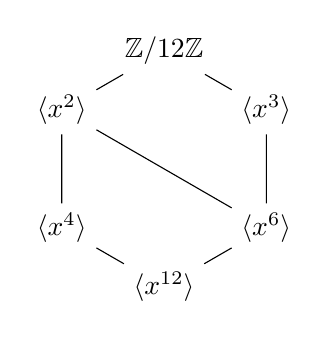
\begin{tikzpicture}[scale=1]
  \node (one) at (90:1.5cm) {$\Z/12\Z$};
  \node (b) at (150:1.5cm) {$\cyc{x^2}$};
  \node (a) at (210:1.5cm) {$\cyc{x^4}$};
  \node (zero) at (270:1.5cm) {$\cyc{x^{12}}$};
  \node (c) at (330:1.5cm) {$\cyc{x^6}$};
  \node (d) at (30:1.5cm) {$\cyc{x^3}$};
  \draw (zero) -- (a) -- (b) -- (one) -- (d) -- (c) -- (zero);
  \draw (b) -- (c);
\end{tikzpicture}
\end{minipage}
\phantom{spacingyeAHoo}
\begin{minipage}{.2\textwidth}
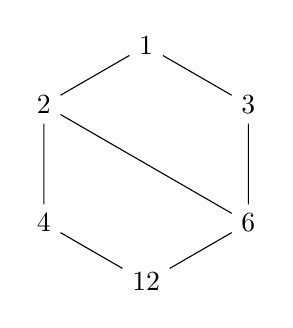
\begin{tikzpicture}[scale=1]
  \node (one) at (90:1.5cm) {$1$};
  \node (b) at (150:1.5cm) {$2$};
  \node (a) at (210:1.5cm) {$4$};
  \node (zero) at (270:1.5cm) {$12$};
  \node (c) at (330:1.5cm) {$6$};
  \node (d) at (30:1.5cm) {$3$};
  \draw (zero) -- (a) -- (b) -- (one) -- (d) -- (c) -- (zero);
  \draw (b) -- (c);
\end{tikzpicture}
\end{minipage}
\qquad\qquad\qquad\qquad
\end{center}
% Z/12Z -- x^2
% Z/12Z -- x^3
% x^2 -- x^4
% x^2 -- x^6
% x^3 -- x^6
% x^6 -- x^12=1
% x^4 -- x^12
% have fun tikzing

For any $\Z/n\Z$, the graph of lattices is dual to the lattice of divisors of $n$, which is shown to the right for $n=12$ in the above figure. % There is a correspondence between the lattice of subgroups of $\Z/n\Z$ and the lattice of divisors of $n$.

\begin{theorem}{}{}
If $H < K$ is a proper subgroup, and if $x \in K - H$ and $\cyc{H \cup \{x\}} = K$, then there are no subgroups properly between $H$ and $K$.
\end{theorem}
% 1--2, 1--3, 2--6,2--4,4--12,6--12

\section{Group actions}
\subsection{Definition of a group action}
\begin{definition}{}{}
A \textbf{group action} $F$ of a group $(G,\times )$ on a set $A$ is a function $F : G\times A \to A$ satisfying two axioms:\footnote{The function application will be $F(g,a)$ for $g \in G$ and $a \in A$. The textbook (Dummit and Foote) writes $g\cdot a$ as notation for $F(g,a)$.}
\begin{itemize}
\item For all $g_1,g_2 \in G$, $a\in A$, then $F(g_2,F(g_1,a)) = F(g_2g_1,a)$.
\item For all $a \in A$, $F(e_G,a) = a$ where $e_G$ is the identity element in $G$.
\end{itemize} 
\end{definition}
\begin{example}{}{}
Here are some examples of group actions:
\begin{enumerate}
\item Let $G = (\R - \{0\},\times)$ be a multiplicative group, and let $A = \R^3$. Define the group action $F$ to be scalar multiplication as follows: $$F(r,(x,y,z)) = (rx,ry,rz)$$
Why is this a group action? We'll check that the two axioms hold. Indeed, the functions compose, i.e., for $r,s\in G$, then $F(r,F(s,(x,y,z))) = (rsx,rsy,rsz)$.\footnote{Using the textbook notation, we can write $r\cdot (s\cdot (x,y,z)) = (rs)\cdot (x,y,z)$.} Furthermore, $F(1,(x,y,z)) = (1x,1y,1z) = (x,y,z)$ as desired.
\item Let $G = S_n$ be the group of permutations on $n$ elements. Then, let $A = \{ 1,2,\ldots,n \}$. Define $F : S_n \times A \to A$ by $F(\sigma,j) = \sigma(j)$. This is also a group action.
\item Let $G = \{ [\begin{smallmatrix} \cos\theta & -\sin\theta \\
\sin\theta & \cos\theta \end{smallmatrix}] \}$ under matrix multiplication be the group of rotation matrices in the Euclidean two-dimensional plane. For brevity, we'll write $R(\theta) = [\begin{smallmatrix} \cos\theta & -\sin\theta \\
\sin\theta & \cos\theta \end{smallmatrix}]$. This is a group because:
	\begin{enumerate}
	\item \textit{Inverses} - for any rotation $R(\theta)$, take $R(-\theta)$.
	\item \textit{Identity} - let the identity $R(0) = [\begin{smallmatrix} 1 & 0 \\ 0 & 1 \end{smallmatrix}]$.
	\item \textit{Closure} - for any $R(\alpha)$ and $R(\beta)$, $R(\alpha)R(\beta) = R(\alpha + \beta)$.
	\end{enumerate}
Furthermore, this group inherits associativity from matrix multiplication.
\end{enumerate}
\fakeline
\end{example}
\vspace{-.5cm}
\subsection{Geometric rotations as group actions}
Consider a geometric figure as a subset $S \subseteq \R^2$ in the real plane.
\begin{definition}{}{}
Given a set $X$, the \textbf{power set} $P(X)$ is defined to be the collection of all subsets of $X$. 
\end{definition}
Let $X = \{  1,2,\ldots,n \}$. Then $P(X)$ has $2^n$ elements, because for each element of $X$, it can either be included or not be included in a given subset of $X$. For example, we have $\{ 1,2 \} \in P(X)$, $\emptyset \in P(X)$, and so on.

Now, let's define a group action on the power set. Define $F : G \times P(\R^2) \to P(\R^2)$ by $F(M,S) = M(S)$ where $M$ is the rotation matrix $M \in G$ and $S$ is our geometric figure in $\R^2$. Note that $M(S) = \{ Ms \in \R^2 : s \in S \}$.

To see what this looks like, let $R(\frac{\pi}{2}) = [\begin{smallmatrix} 0 & -1 \\ 1 & 0 \end{smallmatrix}]$. This will rotate $S \subseteq \R^2$ counterclockwise by $\pi/2$. Exercise: check that this is a group action.

\subsection{Permutations and group actions}
\begin{theorem}{}{}\label{permtheorem}
Let a group $G$ act on a set $A$ via the group action $F$. Then, define $\sigma_g$ by $a \mapsto F(g,a)$. We claim that this $\sigma_g$ is a permutation in $S_A$.
\end{theorem}
\begin{proof}
We need to show that $\sigma_g : A \to A$ is both injective and surjective. Indeed, to show injectivity, take any $a_1,a_2 \in A$. Suppose $\sigma_g(a_1) = \sigma_g(a_2)$. Then:
\begin{align*}
a_1 &= e \cdot a_1 \\
&= (g^{-1}g)\cdot a_1 \\
&= g^{-1}\cdot (g \cdot a_1) \\
&= g^{-1}\cdot (g\cdot a_2) \\
&= (g^{-1}g)\cdot a_2 \\
&= a_2
\end{align*}
This is sufficient to show injectivity, since $\sigma_g(a_1) = \sigma_g(a_2) \implies a_1 = a_2$. Next up, we'll show surjectivity. Take any element $a \in A$; then, we want to find $a' \in A$ such that $\sigma_g(a') = a$. Consider $g^{-1}\cdot a \in A$; then $g \cdot (g^{-1}a) = (gg^{-1})\cdot a = a$. Thus, $\sigma_g$ as defined above is both surjective and injective, and therefore bijective. Woohoo!
\end{proof}

You can find some of the algebraic structure of $G$ in $S_A$; specifically, the homomorphism is preserved. This is defined formally in the following theorem. Note that this does not necessarily preserve injectivity.
\begin{theorem}{}{}
Let $(G,\times)$ act on a set $A$, such that the group action is defined as follows:
\begin{align*}
\varphi : \ &G\to S_A \\
&g\mapsto \sigma_g
\end{align*}
where $\sigma_g$ is defined as in Theorem \ref{permtheorem}. Then $\varphi$ is a homomorphism.
\end{theorem}
\begin{proof}
Consider any two elements $g_1,g_2 \in G$. We need to check that $\varphi(g_1)\varphi(g_2) = \varphi(g_1g_2)$. Indeed, for any $a\in A$, we have
\begin{align*}
\sigma_{g_1}\sigma_{g_2}(a) &= \sigma_{g_1}(\sigma_{g_2}(a)) \\
&= g_1 \cdot (g_2 \cdot a) \\
&= (g_1g_2) \cdot a \\
&= \sigma_{g_1g_2}(a)
\end{align*}
Thus $\varphi(g_1)\varphi(g_2) = \varphi(g_1g_2)$ as desired.
\end{proof}

%4  quotient groups
\section{Quotient groups}
%Idea of quotients: suppose $\phi : G\to H$ homomorphism. remember that homomorphisms aren't necessarily surjective (cartoon lines to dots, not all points hit because not necessarily surjective).
\subsection{Fibers and cosets}
\begin{definition}{}{}
The \textbf{image} of $\varphi$ is $\operatorname{im}(\varphi) = \{ \varphi(g) : g \in G \}$.
\end{definition}

\begin{definition}{}{}
The \textbf{kernel} of $\varphi$ is $\operatorname{ker}(\varphi) = \{ g \in G : \varphi(g) = 1_H \}$.
\end{definition}

\begin{theorem}{}{}
Let $\varphi : G \to H$ be a group homomorphism. Then $\operatorname{ker}(\varphi) \le G$ is a subgroup.
\end{theorem}
\begin{proof}
Note that $\varphi(1_G) = \varphi(1_H)$, so $1_G \in \operatorname{ker}(\varphi)$. Now, given $x,y \in \operatorname{ker}(\varphi)$, check that $xy^{-1} \in \operatorname{ker}(\varphi)$ by the subgroup criterion. Indeed, since $\varphi$ is a homomorphism, $\varphi(xy^{-1}) = \varphi(x)\varphi(y)^{-1} = 1_H(1_H)^{-1} = 1_H$.
\end{proof}
\begin{theorem}{}{}
Let $\varphi : G \to H$ be a group homomorphism. Then $\operatorname{im}(\varphi) \le H$ is a subgroup.
\end{theorem}
\begin{definition}{}{}
Let $\varphi : G\to H$ be a homomorphism. Then given $h \in \operatorname{im}(\varphi)$, we say the \textbf{fiber} over $h$ is $$\varphi_h = \{ g \in G : \varphi(g) = h \}$$
\end{definition}
For example, $\varphi_{1_H} = \operatorname{ker}(\varphi)$. The fibers of $\varphi$ partition $G$, i.e., every element of $G$ is in exactly one fiber. We'll see this again with left and right cosets of a subgroup.

\begin{definition}{}{}
Let $\varphi : G \to H$ be a group homomorphism. Then define $G/\text{ker}(\varphi)$ to have elements as the fibers of $\varphi$. Then we define $\varphi_h\cdot\varphi_{h'}=\varphi_{hh'}$ to be the group operation.
\end{definition}
Note that $G/\text{ker}(\varphi) \cong \text{im}(\varphi)$.

\begin{definition}{}{}
Let $H$ be any subgroup of $G$. Then the $\textbf{left cosets}$ of $H$ are subsets of the form $gH = \{ gh : h \in H \}$. The $\textbf{right cosets}$ of $H$ are subsets of the form $Hg = \{ hg : h \in H \}$.
\end{definition}
Further, remark that $H = 1H$ is a left coset, but it's the only left coset that's a subgroup because it is the only one containing the identity element $1 \in G$. Similarly, $H=H1$ is the only right coset that is a subgroup.

\begin{example}{}{}\label{ex:cosets}
Let $G = D_8$ be the group of symmetries of a square with the following eight elements: $\{ 1,r,r^2,r^3,s,sr,sr^2,sr^3 \}$. Furthermore, let $H = \{ 1,r,r^2,r^3 \}$ be the subgroup of rotations. The left cosets are as follows:
\begin{multicols}{2}
\begin{itemize}
\item $H = \{ 1,r,r^2,r^3 \}$
\item $rH = \{ r,r^2,r^3,1 \}$
\item $r^2H = \{ r^2,r^3,1,r \}$
\item $r^3H = \{ r^3,1,r,r^2 \}$
\end{itemize}
\begin{itemize}
\item $sH = \{ s,sr,sr^2,sr^3 \}$
\item $srH = \{ sr,sr^2,sr^3,s \}$
\item $sr^2H = \{ sr^2,sr^3,s,sr \}$
\item $sr^3H = \{ sr^3,s,sr,sr^2 \}$
\end{itemize}
\end{multicols}
Of these left cosets, only two ($H$ and $sH$) are distinct. Note that the left cosets of $H$ partition $G$, since every element of $G$ is contained in exactly one of $H$ and $sH$.
\end{example}

\begin{theorem}{}{}
The left cosets of $H$ partition $G$.\footnote{The right cosets behave similarly, but there is no guarantee that the partitions are the same.}
\end{theorem}
\begin{proof}
Given $g\in G$, note that $g = g1 \in gH$, so every element of $G$ appears in at least one left coset of $H$. Now, we need to show that these cosets are disjoint. To prove this, suppose $g \in g'H$. Then, it suffices to show that $gH = g'H$. Indeed, let $g = g'h'$ for some $h' \in H$. Then:
\begin{align*}
gH &= \{ gh : h \in H \} \\
&= \{ g'h'h : h \in H \} \\
&= g'H \text{ (since $h'H = H$ by closure and inverses)}
\end{align*}
Therefore, the left cosets of $H$ are indeed distinct.
\end{proof}

\begin{theorem}{}{}
Let $\varphi : G \to H$ be a homomorphism. For $g \in G$, let $h = \varphi(g)$. Then: $$\varphi_h = gK =Kg$$
where $K=\text{ker}(\varphi)$.
\end{theorem}

\begin{lemma}{}{}
Given a subgroup $H \le G$, there is a bijection from $H \to gH$ for any $g\in G$.\footnote{Similarly for the right coset $Hg$.}
\end{lemma}
\begin{proof}
Consider the following map (not necessarily a homomorphism):
\begin{align*}
f : \ &H \to gH \\
&h \mapsto gh
\end{align*}
Indeed, $f$ is a bijection from $H$ to $gH$ as defined above.
\end{proof}
\begin{corollary}{Lagrange's Theorem}{}
Let $G$ be a finite group, with subgroup $H \le G$. Then $|H|$ divides $|G|$.
\end{corollary}
\begin{proof}
$G$ is partitioned into cosets $H,g_2H, \ldots,g_kH$ for some $g_2,\ldots,g_k$. We write 
\begin{align*}
|G| &= |H| + |g_2H| + \cdots + |g_kH| \\
&= |H| + \cdots + |H| \\
&= k|H|
\end{align*}
so indeed the order of $G$ is a multiple of $|H|$.
\end{proof}

\begin{definition}{}{}
A subgroup $N$ of $G$ is \textbf{normal} if $gN = Ng$ for all $g \in G$. In this case, we write $H \trianglelefteq G$.
\end{definition}

\begin{example}{}{}
If $G$ abelian, then any subgroup of $G$ is normal. However, is the reverse statement true? No, consider $H = \{ 1,r,r^2,r^3 \} \le D_8$ as discussed in Example \ref{ex:cosets}. $H$ is normal in $G$, but we know that $G = D_8$ is not abelian since $rs \ne sr$, for example.

To see an example of a non-normal subgroup, consider $H' = \cyc{s} = \{ 1,s \} \le D_8$. The left and right cosets of $H'$ are as follows:
\vspace{-0.15cm}
\begin{multicols}{2}
\begin{itemize}
\item $H' = \{ 1,s \}$
\item $rH' = \{ r,sr^3 \}$
\item $r^2H' = \{ r^2,sr^2 \}$
\item $r^3H' = \{ r^3,sr \}$
\end{itemize}
\begin{itemize}
\item $H' = \{ 1,s \}$
\item $H'r = \{ r,sr \}$
\item $H'r^2 = \{ r^2,sr^2 \}$
\item $H'r^3 = \{ r^3,sr^3 \}$
\end{itemize}
\end{multicols}
\vspace{-0.3cm}
Indeed, these left and right cosets are not the same, so $H'$ is not a normal subgroup of $G$. 
\end{example}
\newpage
\subsection{Conjugacy and normality}
\begin{definition}{}{}
An \textbf{automorphism} of $G$ is an isomorphism $G \to G$.
\end{definition}
\begin{definition}{}{}
Let $G$ be a group with element $g \in G$. Then \textbf{conjugation} by $g$ is the following automorphism:
\begin{align*}
\varphi : \ &G \to G \\
&x\mapsto gx{g^{-1}}
\end{align*}
\end{definition}
\begin{proof}
We'll show that $\varphi$  (conjugation) is indeed an isomorphism in three steps:
\begin{enumerate}[ i. ]
\item To show that $\varphi$ is a homomorphism:
\begin{align*}
\varphi(xy) &= gxyg^{-1} \\
&= gxg^{-1}gyg^{-1} \\
&= \varphi(x)\varphi(y)
\end{align*}
\item To show that $\varphi$ is injective, take $x,y \in G$ such that $gxg^{-1} = gyg^{-1}$. Then we have $x=y$ as desired.
\item To show that $\varphi$ is surjective, let $y\in G$, and note $\varphi(g^{-1}yg) = g(g^{-1}yg)g^{-1} = y$.
\end{enumerate}
\end{proof}

\begin{definition}{}{}
Two elements $x,y \in G$ are \textbf{conjugates} if $y = gxg^{-1}$ for some $g \in G$.
\end{definition}
\begin{theorem}{}{}
Conjugacy is an equivalence relation on $G$.
\end{theorem}
\begin{proof}
By the definition of equivalence relations:
\begin{enumerate}[ i. ]
\item \textbf{Reflexive} - $g = 1g1^{-1}$ for all $g \in G$.
\item \textbf{Symmetric} - say $y = gxg^{-1}$. Then $g^{-1}yg = x$, so this relation is symmetric.
\item \textbf{Transitive} - say $y = gxg^{-1}$ and $z=hyh^{-1}$ for some $g,h \in G$. Then $z = h(gxg^{-1})h^{-1} = (hg)x(hg)^{-1}$ as desired.
\end{enumerate}
\end{proof}
\begin{definition}{}{}
Let $G$ be a group. The \textbf{conjugacy classes} of $G$ are the equivalence classes under the relation of conjugacy.
\end{definition}
\begin{example}{}{}\label{ex:conjugacy}
For example, consider the conjugacy classes of $D_8$:
\begin{itemize}
\item $\{1\}$ as the identity
\item $\{r^2\}$ since $sr^2s^{-1} = r^2ss^{-1} = r^2$
\item $\{r,r^3\}$ since $srs^{-1} = r^3ss^{-1} = r^3$
\item $\{ s, sr^2 \}$ by similar reasoning
\item $\{ sr, sr^3 \}$ by similar reasoning
\end{itemize}
\fakeline
\end{example}
\begin{theorem}{}{}
Let $N \le G$ be a subgroup. Then $N$ is normal if and only if $gNg^{-1} = N$ for all $g \in G$, where we define $gNg^{-1} := \{ gng^{-1} : n\in N \}$.
\end{theorem}
\begin{proof}
Let $N \le G$. Then by definition, $N$ is normal iff $gN = Ng$ for all $g \in G$. Multiplying by $g^{-1}$ on both sides gives $gNg^{-1} = N$ as desired.
\end{proof}
Equivalently, $N \le G$ is normal iff it is a union of conjugacy classes. We can see this by examining unions of the conjugacy classes of $D_8$ as defined in Example \ref{ex:conjugacy}.

\begin{theorem}{Normality Criterion}{}\label{nc}
If $N \le G$ and $gNg^{-1} \subseteq N$ for all $g\in G$, then $N$ is normal.
\end{theorem}
\begin{proof}
We want to show that for all $g \in G$, then $N \subseteq gNg^{-1}$. Indeed, given $n \in N$, write $n = g(g^{-1}ng)g^{-1}$ and note that $g^{-1}ng \in g^{-1}Ng \subseteq N$ by applying the hypothesis to $g^{-1}$.
\end{proof}
\begin{lemma}{}{}
Let $H \le G$ be any subgroup of $G$. Given $g,g' \in G$, then $gH = g'H$ iff $g'\in gH$.
\end{lemma}
\begin{proof}
($\implies$) Since $gH = g'H$, then $g'=g'\cdot 1 \in g'H = gH$ since $1 \in H$.

($\impliedby$) Choose $g' \in gH \cup g'H$, so $gH = g'H$ since left cosets partition $G$.
\end{proof}

\subsection{Quotients}
\begin{definition}{}{}
Let $G$ be a group and $N \trianglelefteq G$ a normal subgroup. The \textbf{quotient group} $G/N$ has the left cosets of $N$ as its elements; further, the binary operation is given as: $$(gN)(hN) = (gh)N$$
\end{definition}
\begin{theorem}{}{}
The binary operation on quotients is well-defined and produces a group.
\end{theorem}
\begin{proof}
To show well-definedness, suppose $gN = g'N$ and $hN = h'N$. Then, we want to show that $(gh)N = (g'h')N$. We have $g' \in gN$ and $h' \in hN$ by the lemma, i.e., $g' = g\cdot n_1$ and $h' = h\cdot n_2$ for $n_1,n_2 \in N$. Again by the lemma, it suffices to show that $g'h' \in (gh)N$. Indeed:
\begin{align*}
g'h' &= g(n_1h)n_2 \\
&=g(hn_1')n_2 \text{ for some $n_1' \in N$}
\end{align*}
since $N$ normal (so $Nh = hN$). Therefore, $g'h' = ghN$ as desired. Now, we want to show that $G/N$ is a group. We'll check the three group axioms:
\begin{itemize}
\item \textbf{Associativity} - by associativity in $G$ and multiplication of left cosets:
\begin{align*}
(g_1Ng_2N)g_3N &= (g_1g_2N)(g_3N) \\
			    &= (g_1g_2)g_3N \\
			    &= g_1(g_2g_3)N \\
			    &= g_1N(g_2Ng_3N)
\end{align*}
\item \textbf{Existence of identity} - the identity element is $N$. Indeed, we can check this as follows: $N \cdot gN = (1g)N = gN = gN\cdot N$.
\item \textbf{Existence of inverses} - $(gN)(g^{-1}N) = (g^{-1})(gN) = N$ as desired.
\end{itemize}
Hence, $G/N$ with the defined binary operation $(gN)(hN) = (gh)N$ is indeed a group.
\end{proof}
\vspace{0.5cm}
\begin{example}{}{}
Let $G = \Z$, so every subgroup of $G$ is normal. In fact, every subgroup is of the form $N = n\Z = \{ \ldots,-2n, -n, 0, n, 2n, \ldots \}$. The cosets of $n\Z$ are $\{ 0+n\Z, 1+n\Z, \ldots, (n-1) + n\Z \}$, i.e., the elements of $Z/n\Z$. \footnote{In additive notation, cosets are often denoted $g+N$ or $N+g$.} For example, the cosets of $5\Z$ are listed below:
\begin{multicols}{3}
\begin{itemize}
\item $0 + 5\Z$
\item $1 + 5\Z$
\item $2 + 5\Z$
\item $3 + 5\Z$
\item $4 + 5\Z$
\end{itemize}
\end{multicols}
which are precisely the elements of $\Z/5\Z$ with addition: $(a+5\Z) + (b+5\Z) = (a+b) + 5\Z$. That is, we wrote $\bar{a} + \bar{b} = \overline{a+b}$.
\end{example}
\begin{theorem}{}{}
Let $\varphi : G \to H$ be a homomorphism, and $K = \operatorname{ker}\varphi = \{ g \in G : \varphi(g) = 1_H \}$. Then:
\begin{enumerate}[ i. ]
\item $K \trianglelefteq G$
\item The left (equivalently, right) cosets of $K$ are the fibers of $\varphi$.
\end{enumerate}
\end{theorem}
\begin{proof}
This follows from the Normality Criterion:
\begin{enumerate}[i.]
\item Given $x \in K$ and $g\in G$, we want to show that $gxg^{-1} \in K$. Indeed, $\varphi(gxg^{-1}) = \varphi(g)\varphi(x)\varphi(g)^{-1} = 1_H$, so $gxg^{-1} \in K$ as desired.
\item Given $g \in G$, let $h = \varphi(g)$. We need to show that $gK = Kg = \varphi_h$. Indeed, given $x \in K$, $\varphi(gx) = \varphi(g)\varphi(x) = \varphi(g) = h$. So $gK \subseteq \varphi_h$. The reverse inclusion is similar.
\end{enumerate}
\end{proof}
Given $N \trianglelefteq G$, there is a natural projection given by the following:
\begin{align*}
\pi : \ &G \to G/N \\
&g \mapsto gN
\end{align*}
Note that $\pi(gg') = (gg')N = (gN)(g'N) = \pi(g)\pi(g')$. Furthermore, $\operatorname{ker}\pi = N$. Remark that a subgroup $N \le G$ is normal if it is the kernel of some homomorphism $G \to H$ from $G$ to some arbitrary group $H$. This is stated formally below.
\begin{theorem}{First Isomorphism Theorem}{}
If $\varphi : G \to H$ is a homomorphism, then $G/\operatorname{ker}\varphi \cong \operatorname{im}\varphi$.
\end{theorem}
\begin{proof}
Define a homomorphism $G/\operatorname{ker}\varphi \to \operatorname{im}\varphi$ by $g(\operatorname{ker}\varphi) = \varphi(g)$. Showing that this homomorphism is an isomorphism is left as an exercise to the reader.
\end{proof}
\begin{definition}{}{}
Let $H \le G$ be any subgroup. Write $|G:H|$ for the \textbf{index} of $H$, i.e., the number of left cosets of $H$ in $G$.\footnote{Or, equivalently, the number of right cosets.}
\end{definition}
Note that if $N \trianglelefteq G$, then $|G/N| = |G:N|$ by Lagrange's Theorem. Let $N \trianglelefteq G$: how does the lattice of subgroups of $G/N$ compose to that of $G$? 

For example, let $G = \Z$ and $N = 12\Z = \{ \ldots,-12,0,12,\ldots \}$. Then, consider the lattice of subgroups for $\Z$ and the lattice of subgroups for $\Z/12\Z$:
\begin{center}
\begin{minipage}{.2\textwidth}
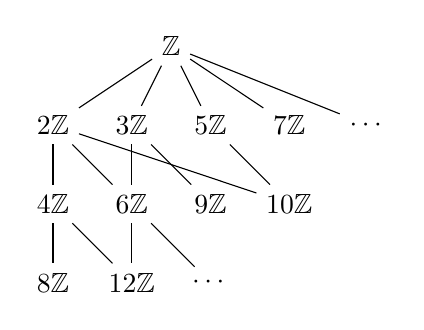
\begin{tikzpicture}[scale=1]
  \node (one) at (0,0) {$\Z$};
  \node (b) at (-1.5,-1) {$2\Z$};
  \node (a) at (-0.5,-1) {$3\Z$};
  \node (zero) at (0.5,-1) {$5\Z$};
  \node (c) at (1.5,-1) {$7\Z$};
  \node (more) at (2.5,-1) {$\cdots$};
  \node (d) at (-1.5,-2) {$4\Z$};
  \node (e) at (-.5,-2) {$6\Z$};
  \node (f) at (.5,-2) {$9\Z$};
  \node (g) at (1.5,-2) {$10\Z$};
  \node (h) at (-1.5,-3) {$8\Z$};
  \node (i) at (-.5,-3) {$12\Z$};
  \node (moretwo) at (0.5,-3) {$\cdots$};
  \draw (one) -- (b);
  \draw (one) -- (a);
  \draw (one) -- (zero);
  \draw (one) -- (c);
  \draw (one) -- (more);
  \draw (b) -- (d);
  \draw (b) -- (e);
  \draw (b) -- (g);
  \draw (a) -- (e);
  \draw (a) -- (f);
  \draw (zero) -- (g);
  \draw (d) -- (h);
  \draw (d) -- (i);
  \draw (e) -- (i);
  \draw (e) -- (moretwo);
\end{tikzpicture}
\end{minipage}
\phantom{spacingyeAHaa}
\begin{minipage}{.2\textwidth}
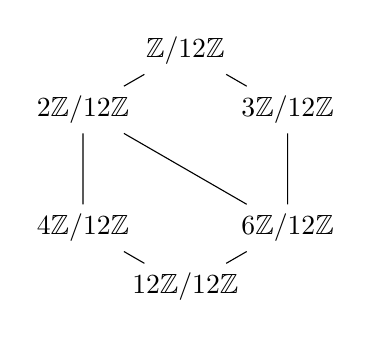
\begin{tikzpicture}[scale=1]
  \node (one) at (90:1.5cm) {$\Z/12\Z$};
  \node (b) at (150:1.5cm) {$2\Z/12\Z$};
  \node (a) at (210:1.5cm) {$4\Z/12\Z$};
  \node (zero) at (270:1.5cm) {$12\Z/12\Z$};
  \node (c) at (330:1.5cm) {$6\Z/12\Z$};
  \node (d) at (30:1.5cm) {$3\Z/12\Z$};
  \draw (zero) -- (a) -- (b) -- (one) -- (d) -- (c) -- (zero);
  \draw (b) -- (c);
\end{tikzpicture}
\end{minipage}
\end{center}
\begin{lemma}{}{}
Let $K \le G$ with $N \trianglelefteq K$. Then $K$ is a union of cosets of $N$.
\end{lemma}
\begin{proof}
Given $n \in N$ and $x \in K$, we have $xnx^{-1} \in N$ since $x \in G$ and $N$ normal. Then, $K/N = \{ kN : k \in K \}$ is a group, and we claim $K/N \le G/N$. The group structure on $K/N$ comes from that of $G/N$.
\end{proof}
\begin{theorem}{Third Isomorphism Theorem}{}
Say $N \trianglelefteq G$, $K\trianglelefteq G$, and $N \le K$. Then $K/N \trianglelefteq G/N$ and $(G/N)/(K/N) \cong G/K$.
\end{theorem}
\begin{proof}
First, we'll show that $K/N \trianglelefteq G/N$. Given $kN \in K/N$ and $gN \in G/N$. We want to show that $(gN)(kN)(gN)^{-1} \in K/N$. Indeed, $(gN)(kN)(gN)^{-1} = (gkg^{-1})N \in K/N$ by normality of $K$ in $G$.

To show that $(G/N)/(K/N) \cong G/K$, we'll use the first isomorphism theorem. Indeed, let's define the following map and show it's a homomorphism as follows:
\begin{align*}
\varphi : \ &G/N \to G/K \\
&gN \mapsto gK
\end{align*}
First, check that $\varphi$ is well-defined as follows: given $gN = g'N$, we want to show $gK = g'K$. Indeed, $g' \in gN \subseteq gK$, so $gK = g'K$ as desired. Next, we'll check that $\varphi$ is a homomorphism:
\begin{align*}
\varphi(gNg'N) &= \varphi((gg')N) \\
&= gg'K \\
&= gKg'K \\
&= \varphi(gN)\varphi(g'N)
\end{align*}
Now, we'll show that $\varphi$ is surjective. Indeed, given any element of $gK \in G/K$ for some $g \in G$, note that $\varphi(gN) = gK$. Showing this is surjective means that $\operatorname{im}\varphi = G/K$.

Finally, note that $\operatorname{ker}\varphi = \{ gN : gK = K \} = \{ gN : g\in K \} = K/N$. Applying the first isomorphism theorem gives $(G/N)/(K/N) \cong G/K$.
\end{proof}
\vspace{0.5cm}
\begin{example}{}{}
For example, we'll show that $\Z/3\Z \cong (\Z/6\Z)/(3\Z/6\Z)$. Indeed, consider the elements of these sets:
\begin{itemize}
\item $\Z/6\Z = \{ 6\Z, 1+6\Z, 2+6\Z, 3+6\Z, 4+6\Z, 5+6\Z \}$
\item $3\Z/6\Z = \{ 6\Z, 3+6\Z \}$
\end{itemize}
Then, say any two elements $x,y \in \Z/6\Z$ are equivalent iff $x - y \in 3\Z/6\Z$. The equivalence classes on this relation are precisely the elements of $\Z/3\Z$:
\begin{itemize}
\item $6\Z + 3\Z/6\Z = 3+6\Z + 3\Z/6\Z = \{ 6\Z, 3+6\Z \}$
\item $1+6\Z + 3\Z/6\Z = 4+6\Z + 3\Z/6\Z = \{ 1+6\Z, 4+6\Z \}$
\item $2+6\Z + 3\Z/6\Z = 5+6\Z + 3\Z/6\Z = \{ 2+6\Z, 5+6\Z \}$
\end{itemize}
\fakeline
\end{example}

\begin{theorem}{Fourth Isomorphism Theorem (Lattice Isomorphism)}{}
Let $N \trianglelefteq G$. There is a bijective map 
\begin{align*}
\Phi : \ &\{\text{subgroups of } G \text{ containing } N\} \to \{\text{subgroups of } G/N\} \\
&H \mapsto H/N
\end{align*}
It is inclusion preserving and normality preserving. That is, $K \trianglelefteq G$ iff $K/N \trianglelefteq G/N$, and in this case $(G/N)/(K/N) \cong G/K$.
\end{theorem}
\begin{proof}
We'll construct an inverse to $\Phi$. Given $\bar{H} \le G/N$, let $H = \{ g \in G : gN \in \bar{H} \}$. Claim that $H$ is a subgroup, and $H/N = \bar{H}$. To show this is inclusion-preserving, show that if $H \le H'$ then $H/N \le H'/N$.
\end{proof}
\begin{theorem}{Second Isomorphism Theorem}{}
Let $G$ be a group, with subgroups $A, N \le G$. Then define the subset $$AN = \{ an : a\in A, n\in N \}$$ which need not be a subgroup. Then, if $A \le G$ and $N \trianglelefteq G$:
\begin{enumerate}[ i. ]
\item $AN \le G$
\item $AN/N \cong A/A\cap N$
\end{enumerate}
Further, remark that $AN = \bigcup_{a\in A} aN$.
\end{theorem}
\begin{proof}
First, we'll show that $AN$ is a subgroup. Indeed, $1 \in AN$. Given $a_1,a_2 \in A$ and $n_1,n_2 \in N$, then we want to show $$(a_1n_1)(a_2n_2)^{-1} \in AN$$
Indeed, $(a_1n_1)(a_2n_2)^{-1} = a_1(n_1n_2^{-1}a_2^{-1}) = a_1a_2^{-1}n$ for some $n \in N$ (since $a_2^{-1}N = Na_2^{-1}$). So $(a_1n_1)(a_2n_2)^{-1} \in AN$.

For the second part of this theorem, we'll use the first isomorphism theorem. Say: 
\begin{align*}
\varphi : \ &A \to AN/N \\
&a \mapsto aN
\end{align*}
is a surjective homomorphism (proof as exercise). Then, $\operatorname{ker}\varphi = \{ a \in A : aN = N \} = A \cap N$. So we're done by the first isomorphism theorem.
\end{proof}

\subsection{Composition series and the Jordan Holder Theorem}
For the sake of analogy, recall prime factorization in $\Z$: given $n \in \Z$ with $n > 1$, then $n$ has a factorization $p_1^{\alpha_1}\cdot p_2^{\alpha_2}\cdots p_k^{\alpha_k}$ where $p_i \ne p_j$ if $i \ne j$; this factorization is unique up to reordering of the prime powers.
\begin{theorem}{}{}
$mn = \operatorname{gcd}(m,n)\cdot\operatorname{lcm}(m,n)$ for $m,n \ge 1$
\end{theorem}
\begin{definition}{}{}
A nontrivial group $G$ is \textbf{simple} if $1,G$ are the only normal subgroups of $G$.
\end{definition}
\begin{example}{}{}
$\Z/p\Z$ is simple for $p$ prime.
\end{example}
\begin{definition}{}{}
Let $G$ be a nontrivial group. A \textbf{composition series}\footnote{Warning: $N_i$ need not be normal in $G$.} for $G$ is $$1=N_0 \trianglelefteq N_1 \trianglelefteq N_2 \trianglelefteq \cdots \trianglelefteq N_k = G$$
where $N_i \le G$ are subgroups and each quotient $N_{i+1}/N_i$ is simple for $i=0,\ldots,k-1$.\footnote{Saying that $N_{i+1}/N_i$ is simple is equivalent to saying that there are no normal subgroups between $N_i$ and $N_{i+j}$. This is a consequence of the fourth isomorphism theorem.}
\end{definition}
\begin{definition}{}{}
Given a composition series $N_0, \ldots, N_k$, the \textbf{factors} are the quotients $N_{i+1}/N_i$ for $i=0,\ldots,k-1$.
\end{definition}
\begin{example}{}{}
In the dihedral group $D_8$, the composition series is as follows:
$$\{ 1 \}\trianglelefteq \{ 1,s \}\trianglelefteq \{ 1,s,sr^2, r^2 \}\trianglelefteq D_8$$
What are the factors? They are all cyclic of order $2$, i.e., $\Z/2\Z$. However, this is not the only possible example. We can also have the following composition series:
$$\{ 1 \}\trianglelefteq \{ 1,r^2 \}\trianglelefteq \{ 1,r,r^2, r^3 \}\trianglelefteq D_8$$
which has the same factors as the previous composition series.
\end{example}
\begin{theorem}{Jordan Holder Theorem}{}
Let $G$ be a nontrivial finite group. Then:
\begin{enumerate}[ i. ]
\item $G$ has a composition series.
\item Any two composition series for $G$ will have the same factors up to reordering.
\end{enumerate}
(Note that the factors don't determine the group.)
\end{theorem}
\begin{proof}
To show that every nontrivial finite group has a composition series, use strong induction on $|G|$. First, show the statement is true when $|G| = 2$. Then we show that if the statement is true for all $|G| < n$, then it's also true for $|G| = n$. Then the statement is true for all $|G| \ge 2$.

Indeed, if $|G| = 2$, then $G$ is simple, so it has a composition series $1 \trianglelefteq G$. Now, let $|G| = n$: if $G$ is simple, we're done. Therefore, assume there exists some $N$ such that $1 \trianglelefteq N \trianglelefteq G$. Note that $N$ and $G/N$ have order smaller than $G$, so by the inductive hypothesis, there exists a composition series $$1 \trianglelefteq N_1\trianglelefteq \cdots \trianglelefteq N_k = N$$
and there exists a composition series $1 \trianglelefteq N_{k+1}/N \trianglelefteq N_{k+2}/N \trianglelefteq \cdots \trianglelefteq G/N$. So by the fourth isomorphism theorem, we write:
$$1 \trianglelefteq \cdots \trianglelefteq N \trianglelefteq N_{k+1} \trianglelefteq N_{k+2} \trianglelefteq \cdots \trianglelefteq G$$
is a composition series for $G$ as desired. (The second part of this theorem is left as an exercise to the reader.)
\end{proof}

\subsubsection{Alternating groups}

\begin{definition}{}{}
Let $n \ge 1$. Given the set of descents
$$S =  \{ (i,j) : 1 \le i < j \le n, \sigma{i} > \sigma{j} \}$$
Then the \textbf{sign} of a permutation $\sigma \in S_n$ is $(-1)^{|S|}$.
\end{definition}
\begin{example}{}{}
Let's choose an element of $S_5$. Namely, let:
$$\sigma = \begin{pmatrix}
1 & 2 & 3 & 4 & 5 \\
1 & 4 & 3 & 2 & 5 \\
\end{pmatrix}$$
Then $|S| = 3$ is the number of descents of $\sigma$, so $\operatorname{sgn}(\sigma) = (-1)^3 = -1$.
\end{example}
\begin{theorem}{}{}
Every $\sigma \in S_n$ can be written as a product of transpositions (i.e., $2$-cycles).
\end{theorem}
Consider the ``physical proof" of the above theorem. Given a number of elements in any order, you can swap pairs of them until you reach the desired order.
\begin{theorem}{}{}
If $\operatorname{sgn}(\sigma) = 1$, then any expression of $\sigma$ as a product of transpositions contains an even number of transpositions. If $\operatorname{sgn}(\sigma) = -1$, then $\sigma$ is a product of an odd number of transpositions.
\end{theorem}
\begin{proof}
Suppose $\tau$ is an adjacent transposition $\begin{pmatrix} i & i+1 \end{pmatrix}$. Then $\operatorname{sgn}(\sigma) = -\operatorname{sgn}(\tau \cdot \sigma)$. But now, suppose $\tau$ is any transposition: then it can be written as an odd number of adjacent transpositions. Hence $\operatorname{sgn}(\sigma) = -\operatorname{sgn}(\tau \cdot \sigma)$ for the general case.
\end{proof}

\begin{corollary}{}{}
$\operatorname{sgn} : S_n \to \{ \pm 1 \}$ is a (surjective) homomorphism.
\end{corollary}

\begin{definition}{}{}
$A_n = \operatorname{ker}(\operatorname{sgn}) = \{ \sigma \in S_n : \operatorname{sgn}(\sigma) = 1 \}$
\end{definition}

\begin{theorem}{}{}
$A_i$ is simple for $i \ge 5$.
\end{theorem}

\section{Product groups}
\begin{definition}{}{}
Let $G_1$ and $G_2$ be groups. Define the \textbf{product} $$G_1 \times G_2 = \{ (g_1, g_2) : g_1 \in G_1, g_2 \in G_2 \}$$
with binary operation $(g_1,g_2)\cdot (g_1',g_2') = (g_1g_1', g_2g_2')$. This is a group.
\end{definition}
\begin{example}{}{}
$\R \times \R = \R^2$ from HW 1. This can be extended to show that $\R^n = \R \times \cdots \times \R$ ($n$ times). Note that $|G_1 \times \cdots \times G_n| = |G_1| \cdots |G_n|$.

For example, consider the product $\Z/2\Z \times \Z/3\Z = \{ (\bar{0},\bar{0}),(\bar{0},\bar{1}),(\bar{0},\bar{2}),(\bar{1},\bar{0}),(\bar{1},\bar{1}),(\bar{1},\bar{2}) \}$. Claim that this is isomorphic to $\Z/6\Z$:
\begin{center}
\begin{tabular}{c | c c}
$\Z/6\Z$ & $\Z/2\Z$ & $\Z/3\Z$ \\\hline
$\bar{0}$ & $\bar{0}$ & $\bar{0}$ \\
$\bar{1}$ & $\bar{1}$ & $\bar{1}$ \\
$\bar{2}$ & $\bar{0}$ & $\bar{2}$ \\
$\bar{3}$ & $\bar{1}$ & $\bar{0}$ \\
$\bar{4}$ & $\bar{0}$ & $\bar{1}$ \\
$\bar{5}$ & $\bar{1}$ & $\bar{2}$ \\
\end{tabular}
\end{center}
\fakeline
\vspace{0.15cm}
\end{example}
\begin{theorem}{}{}
Given $G_1, G_2$, there are natural projection homomorphisms $$\pi_1 : G_1 \times G_2 \to G_1\text{, } \pi_2 : G_1 \times G_2 \to G_2$$
where $\pi_1(g_1,g_2) = g_1$ and $\pi_2(g_1,g_2) = g_2$. Then given homomorphisms $\varphi_1 : G \to G_2$, $\varphi_2 : G\to G_2$, there exists a unique homomorphism $\varphi : G \to G_1 \times G_2$ making the following diagram commute:

\[ \begin{tikzcd}
G \arrow{r}{\varphi_2} \arrow[swap]{d}{\varphi_1}\arrow{rd}{\varphi} & G_2 \\%
G_1 & G_1 \times G_2\arrow{u}{\pi_2}\arrow{l}{\pi_1}
\end{tikzcd}
\]

In other words, $\pi_1\varphi = \varphi_1$ and $\pi_2\varphi = \varphi_2$.
\end{theorem}
We can apply this theorem to the previous example. Consider the following projection maps:
\begin{align*}
\varphi_1 : \ &\Z/6\Z \to \Z/2\Z \\
\varphi_2 : \ &\Z/6\Z \to \Z/3\Z
\end{align*}
Let $\varphi : \Z/6\Z \to \Z/2\Z \times \Z/3\Z$. In fact, the unique such map is $\varphi(g) = (\varphi_1(g), \varphi_2(g))$ Then we claim that $\varphi$ is an isomorphism:
\begin{itemize}
\item \textbf{Injectivity} - from the table above, the kernel has a single element $\bar{0}$.
\item \textbf{Surjectivity} - follows because the function is injective and maps from finite equal cardinalities.
\item \textbf{Homomorphism} - we defined $\varphi$ as such.
\end{itemize}

\begin{theorem}{Chinese Remainder Theorem}{}
Suppose $n_1,\ldots,n_k \ge 1$ are pairwise relatively prime. Then if $N = \prod n_i$, we have $$\Z/N\Z \cong \Z/n_1\Z \times \cdots \times \Z/n_k\Z$$
\end{theorem}
\begin{example}{}{}
As an exercise: how many students ($n$) are present in abstract algebra?
\begin{align*}
n &\equiv 4\pmod{5} \\
n&\equiv 3\pmod{7}
\end{align*}
\vspace{-0.8cm}
\end{example}
\begin{theorem}{Fundamental theorem of finitely generated abelian groups}{}
Let $G$ be a finitely generated abelian group. Then:
$$G \cong \Z^r \times Z/n_1\Z \times \cdots \times \Z/n_s\Z$$
where $r \ge 0$ and $n_1,\ldots, n_2 \ge 2$ with $n_s\mid n_{s-1}\mid \cdots \mid n_1$. Moreover, this expression for $G$ is unique.
\end{theorem}
Note that the torsion quotient must be isomorphic to $\Z^r$. Up to isomorphism, the finite abelian groups of order $M$ are in bijection with sequences $n_s\mid n_{s-1}\mid\cdots\mid n_1$.

\begin{example}{}{}
The abelian groups of order $8$ are (up to isomorphism):
$$\Z/8\Z\phantom{testing}\Z/4\Z \times \Z/2\Z\phantom{testing}(\Z/2\Z)^3$$
Note that $G \times H \cong H\times G$. The proof of this is left as an exercise to the reader.
\end{example}

\begin{theorem}{}{}
If $G_1, G_2$ are groups, then $G_1 \cong \{ (g_1,1) : g_1 \in G_1 \} \le G_1 \times G_2$. Similarly for $G_2$.
\end{theorem}
\begin{corollary}{}{}
$G_1, G_2 \le G_1 \times G_2$ via the theorem above.
\end{corollary}
Moreover, there exists $H_1, H_2 \le G_1 \times G_2$ with $G_1 \cong G_1$ and $H_2 \cong G_2$. Note also that $H_1 \cap H_2 = 1$ and $H_1H_2 = G_1 \times G_2$. Additionally: $H_1, H_2 \trianglelefteq G_1 \times G_2$.
\begin{theorem}{}{}
Let $G$ be a group, with $H,K \trianglelefteq G$. If $H \cup K = 1$ and $HK = G$, then $G \cong H \times K$.
\end{theorem}
\begin{proof}
Let's define the following function and claim that it is an isomorphism:
\begin{align*}
\alpha : \ &H\times K \to G \\
&(h,k) \mapsto hk
\end{align*}
First, we'll check that $\alpha$ is a homomorphism. Given two elements $(h_1,k_1),(h_2,k_2) \in H\times K$, we can perform the following derivation:
\begin{align*}
\alpha((h_1,k_1)\cdot (h_2,k_2)) &= \alpha((h_1h_2,k_1k_2)) \\
&= h_1h_2k_1k_2 \\
&= h_1k_1h_2k_2 \\
&= [\alpha(h_1,k_1)]\cdot [\alpha(h_2,k_2)]
\end{align*}
Note that this requires $hk = kh$ for all $h \in H$, $k \in K$. Indeed, this is true because $hkh^{-1}k^{-1} \in H \cap K = 1$.

Next, we'll check that $\alpha$ is injective, i.e., $h \in H$ and $k \in K$ such that $hk = 1$, we want to show that $h = k = 1$. Indeed, $h = k^{-1} \in H \cap K = 1$, and $k = 1$ by similar reasoning.

Finally, surjectivity follows from $HK = G$.
\end{proof}
\vspace{0.5cm}
\begin{example}{}{}
$\R^{\times} \cong \R_{> 0} \times \{ \pm 1 \}$ via the above theorem.
\end{example}

\subsection{Semidirect products}
Recall the can of beans from early lectures. Let $R$ denote the symmetry group of the can. Can we say that $R \cong \R/2\pi\Z \times \{ \pm 1 \}$? No, we can't, because $R$ is nonabelian. However, we can say that $R \cong \R/2\pi\Z \rtimes \{ \pm 1 \}$ as follows:
\begin{definition}{}{}
Let $H,K$ be groups and $\varphi : K \to \operatorname{Aut}(H)$ a homomorphism. We define the \textbf{semidirect product group} as follows:
$$G = H \rtimes_{\varphi} K$$
with elements $\{ (h,k) : h \in H, k \in K \}$ and operation $(h_1,k_1)\cdot(h_2,k_2) = (h_1(k_1\cdot h_2), k_1k_2)$ where $(k_1\cdot h_2)$ is the action of $k_1$ on $h_2$ via $\varphi$. More precisely, $k_1 \cdot h_2$ means $\varphi(k_1)(h_2)$.
\end{definition}
As an exercise, check that this is a group! Part of the proof is shown below:
\begin{lemma}{}{}
Inverses exist in the semidirect product group.
\end{lemma}
\begin{proof}
Given an element $(h,k)$, we'll say the inverse is $(k^{-1}h^{-1},k^{-1})$. Indeed:
\begin{align*}
(h,k) \cdot (k^{-1}h^{-1}, k^{-1}) &= (h \cdot k(k^{-1}h^{-1}), kk^{-1}) \\
&= (hh^{-1}, kk^{-1}) \\
&= (1,1)
\end{align*}
so inverses exist as desired. The rest of the proof that the semidirect product is a group is omitted.
\end{proof}
\vspace{0.5cm}
\begin{example}{}{}
Returning to the can of beans, let $G = \R/2\pi\Z$ and $K = \{ \pm 1 \}$. Consider
\begin{align*}
\varphi : \ &K \to \operatorname{Aut}(\R/2\pi\Z) \\
&1 \mapsto \operatorname{id} : H \to H \\
-&1 \mapsto \operatorname{neg} : H \to H
\end{align*}
Claim that $R \cong \R/2\pi\Z \rtimes_{\varphi} \{ \pm 1 \}$, e.g., $(\theta, -1)\cdot (\theta', 1) = (\theta - \theta', -1)$.
\end{example}
Remark that tilde over $H = \{ (h,1) : h \in H \} \trianglelefteq H \rtimes_{\varphi} K$ and tilde over $K = \{ (1,k) : k\in K \} \le H \rtimes_{\varphi} K$ but is not necessarily normal. Further, note:
\begin{align*}
(1,k) \cdot (h,1) \cdot (1,k)^{-1} &= (1(k\cdot h), k)\cdot (1,k^{-1}) \\
&= ((k\cdot h)(k\cdot 1), kk^{-1}) \\
&= (k\cdot h,1)
\end{align*}
so the group action is related to conjugation. We can see this in the following example.

\begin{example}{}{}
For instance, $D_{2n} \cong \Z/n\Z \rtimes \Z/2\Z \cong \{ 1,r,\ldots,r^n \} \rtimes \{ 1,s \}$.
\end{example}
\begin{theorem}{}{}
Let $G$ be a group with $H \trianglelefteq G$ and $K \le G$. If $H \cap K = 1$ and $HK = G$, then $G \cong H \rtimes_{\varphi} K$ with
\begin{align*}
\varphi : \ &K \to \operatorname{Aut}(H) \\
&k \mapsto \Psi_{k} : H \to H \text{ with } \Psi_k(h) = khk^{-1} \text{ (``the conjugation-by-k automorphism")}
\end{align*}
\end{theorem}
\begin{proof}
Consider the following map, which we'll claim is an isomorphism:
\begin{align*}
\alpha : \ &H\rtimes K \to G \\
&(h,k) \mapsto hk
\end{align*}
To check that $\alpha$ is a homomorphism, do the following work:
\begin{align*}
\alpha((h_1,k_1)\cdot (h_2,k_2)) &= \alpha(h_1(k_1 \cdot h_2), k_1k_2) \\
&= \alpha(h_1(k_1h_2k_1^{-1}), k_1k_2) \\
&= h_1(k_1h_2k_1^{-1})k_1k_2 \\
&= h_1k_1h_2k_2 \\
&= \alpha(h_1,k_1) \cdot \alpha(h_2,k_2)
\end{align*}
as desired. We have shown that $\alpha$ is injective and surjective in similar proofs.
\end{proof}
\vspace{0.5cm}
\begin{example}{}{}
Let's return to $D_{2n}$. We'll say $H = \{ 1,r,\ldots,r^{n-1} \} \trianglelefteq D_{2n}$, and say $K = \{ 1,s \}$. Note that $H \cap K = 1$, $HK = D_{2n}$. Finally, $\varphi$ (as in the proposition) is given by
\begin{align*}
s \mapsto \Psi_s : \ &H \to H \\
&r^i \mapsto sr^is^{-1} = r^{-i}
\end{align*}
Then we have that $D_{2n} \cong H \rtimes_{\varphi} K$ as stated in the proposition above.
\end{example}
\subsubsection{Affine transformations}
Let $G$ be the group of invertible affine transformations of $\R^2$, i.e., maps $\R^2 \to \R^2$ expressible as $$x \mapsto Ax + v$$ for $A \in GL_2(\R)$ and $v \in \R^2$ with composition as the group operation. Let $f(x) = Ax + v$ and $g(x) = Bx + w$. Then $(f\circ g)(x) = A(Bx + W) + v = ABx + (Aw + v)$.

Note that $\R^2 \rtimes_{\varphi} GL_2(\R) \cong G$ where $\varphi$ is the natural action of $GL_2(\R)$ on $\R^2$. As an exercise, consider $G$ as an internal\footnote{i..e, as a product of two subgroups congruent to $GL_2(\R), \R^2$} semidirect product group, using propositions in the last subsection.

% SYLOW!! This will all be presented without proof.
\subsection{Sylow theorems}
\begin{definition}{}{}
Suppose $G$ is a group of order $p^{\alpha}\cdot m$ for a prime $p$ with $p \not| \ m$. A \textbf{Sylow $p$-subgroup} of $G$ is a subgroup of order $p^{\alpha}$. Then, let $$Syl_p(G) = \{ \text{Sylow $p$-subgroups} \}$$
and $n_p := |Syl_p(G)|$.
\end{definition}
\begin{theorem}{}{}
Given a group $G$ of order $p^{\alpha} \cdot m$ with $p \not| \ m$, then $n_p \equiv 1 \pmod{p}$ and $n_p \mid m$. In particular, Sylow $p$-subgroups always exist.
\end{theorem}
\begin{theorem}{}{}
Given a group $G$ of order $p^{\alpha} \cdot m$ with $p \not| \ m$, any two Sylow $p$-subgroups $H$ and $H'$ are \textbf{conjugates} (meaning $gHg^{-1} = H'$ for some $g \in G$).
\end{theorem}
\begin{corollary}{}{}
Given a subgroup of $G$ of order $p^{\beta}$ for some $\beta \le \alpha$ and a Sylow $p$-subgroup $K$ of $G$, then $H$ is a subgroup of some conjugate of $K$.
\end{corollary}
\begin{example}{}{}
Let's show that $\Z/10\Z$ and $D_{10}$ are the only groups of order $10$ up to isomorphism. Let $G$ be a group with $|G| = 10$, so the Sylow $p$-subgroups must have orders $2$ or $5$ (the divisors of $10$).

Note that $n_5 \equiv 1 \pmod{5}$ and $n_5\mid 2$, so $n_5 = 1$. Thus $N \trianglelefteq G$ has order $5$. Similarly, $n_2 \equiv 1 \pmod{2}$, and $n_2 \mid 5$, so $n_2 = 1$ or $5$. Indeed, if $n_2 = 1$, then $H \trianglelefteq G$ has order $2$. Then:
$$G \cong H \times N \cong \Z/2\Z \times \Z/5\Z \cong \Z/10\Z$$
by the Chinese Remainder Theorem. In the other case where $n_2 = 5$, then let $H \le G$ have order $2$. Then $G$ is a semidirect product $N \rtimes_{\varphi} H$ for some $\varphi$. Note that $\varphi : \Z/2\Z \to \operatorname{Aut}(\Z/5\Z)$. The only order $2$ automorphisms of $\Z/5\Z$ are $\operatorname{id}$ and $\operatorname{neg}$. If $\varphi(\bar{1}) = \operatorname{id}$, then $G = N\times H \cong \Z/10\Z$. On the other hand, if $\varphi(\bar{1}) = \operatorname{neg}$, then $G \cong D_{10}$.
\end{example}

\end{document}